% Chapter 1

\chapter{Resultados} % Main chapter title
\label{Cap_Res} % For referencing the chapter elsewhere, use \ref{Chapter1} 



\section{Datos recolectados}

%SDatos duros antes del análisis.
Antes de realizar los análisis estadísticos correspondientes para determinar si se encontró -o no- evidencia del Efecto Espejo en nuestros experimentos, los datos recopilados se exploraron de manera exhaustiva, graficando la ejecución de los participantes en relación a diferentes variables.\\ 

%Se destaca la implrtancia de revisar los datos antes de someterlos a analisis estadísticos
Graficar los datos antes de someterlos a un análisis estadístico que guíe la elaboración de conclusiones a partir de los experimentos realizados, constituye una práctica recomendable en tanto que 1) permite evaluar la pertinencia del diseño experimental a la luz de las respuestas registradas y 2) constituye un filtro para descartar la posibilidad de que los participantes estuvieran emitiendo sus respuestas de manera incongruente e inconsistente con las tareas presentadas, permitiendo una mayor confianza en las conclusiones que resulten de su análisis.\\

%Presentación de los controles graficados: Atención, El efecto del paso del tiempo y las variables externas en los estímulos. 
En esta primera sección se presenta un recorrido por las distintas gráficas realizadas con la finalidad de explorar tres grandes fuentes de ruido que, de haber tenido una influencia sobre el desempeño de los participantes, indicarían que estos no respondieron a las tareas planteadas de manera congruente con el propósito de investigación con que se diseñaron los experimentos. Dichas fuentes externas son: 

\begin{enumerate}
\item \textbf{¿Las respuestas se emiten en trenes?} (\textit{Evaluando la atención}).\\

Como un primer filtro se evaluó que los participantes estuvieran poniendo atención a las tareas presentadas al momento de registrar sus respuestas. Para ello se revisaron los patrones con que estas eran emitidas a lo largo de los ensayos.\\

Dado que durante el experimento se presentaron de manera aleatoria estímulos con Ruido o Señal de cualquiera de las dos clases de estímulos diseñadas, se esperaba encontrar una amplia variabilidad en la emisión de respuestas de los participantes (el uso constante de todas las opciones de respuesta facilitadas). De haberse encontrado que los participantes elegían una misma respuesta de manera persistente a lo largo de varios ensayos (trenes de respuesta), habría habido razones para sospechar que no estaban prestando atención a los etímulos que se les presentaron, sino que estuvieron emitiendo sus respuestas en función a aquellas que les precedieron.\\

\item \textbf{¿El Aprendizaje o la Fatiga alteran la ejecución de los participantes?}  (\textit{Evaluando cambios en el desempeño a lo largo del tiempo}).\\

Un segundo filtro estuvo relacionado con la evaluación de los posibles efectos que el paso del tiempo (y el avance entre ensayos) pudo haber tenido sobre el desempeño de los participantes.\\

Por un lado, tomando en cuenta que los experimentos realizados estuvieron conformados por un amplio número de ensayos, a lo largo de los cuales los participantes tuvieron que resolver un par de tareas de detección que podrían haber hecho el procedimiento demasiado demandante, se tenían razones para sospechar que el desempeño de los participantes pudiera verse mermado con el paso de los ensayos, a causa de la Fatiga.\\

Por otro lado, dado que los estímulos incluídos en el experimento estuvieron compuestos por variaciones de una conocida ilusión óptica, se temía que la exposición repetida a la misma redujera su impacto sobre los participantes (por Habituación o Aprendizaje) y su desempeño mejorara considerablemente con el paso del tiempo.\\

\item \textbf{¿Los participantes tienen alguna Preferencia hacia la emisión de ciertas respuestas ante cierto tipo de estímulos?} (\textit{Evaluando el efecto de las variables manipuladas en la construcción de los estímulos}).\\

Un tercer y último filtro se realizó para evaluar el impacto que las variables manipuladas arbitrariamente en la construcción de los estímulos pudieran haber tenido sobre 1) la intensidad de la ilusión óptica presentada y 2) la emisión de respuestas de los participantes.\\

\end{enumerate}

Idealmente, se esperaba que el desempeño registrado de los participantes no presentara ninguna relación con cualquiera de las fuentes de ruido presentadas anteriormente que no fuera la pertenencia de los estímulos a alguna de las clases diseñadas (clase A: figuras de Ebbinghaus con pocos círculos externos; clase B: figuras de Ebbinghaus con más círculos externos).\\












\subsection{Control 1: ¿Los participantes estaban poniendo atención a la tarea al emitir sus respuestas?}

Los experimentos realizados estuvieron compuestos de 640 ensayos, a lo largo de los cuales los participantes tuvieron que 1) decidir si los estímulos presentados cumplían con la condición que se les solicitó detectar y 2) valorar su certidumbre sobre esta primer respuesta y asignarle un puntaje. Dado lo demandante y extenso que fue el procedimiento, una primer preocupación respecto a la fiabilidad de los datos obtenidos tenía que ver con si los participantes estaban -o no- prestando atención a la tarea al momento de registrar sus respuestas -o bien, que en el proceso se agotaran y dejaran de poner atención-. Para evaluar esta posibilidad, se revisaron las respuestas emitidas ensayo a ensayo para verificar que todas las opciones de respuesta fueran utilizadas y que no se presentaran trenes de respuesta (que pudieran sugerir que la emisión de respuestas fue independiente del contenido de la tarea y dependiente de las respuestas emitidas previamente).\\

\begin{itemize}
\item Emisión de respuestas 'Sí/No' a lo largo del experimento.

Primero se graficaron las respuestas emitidas ensayo a ensayo durante la tarea de detección binaria ('Sí, los círculos son iguales' o 'No, los círculos son diferentes'). El objetivo principal de realizar estas gráficas fue el de detectar trenes de respuesta que fueran lo suficientemente largos como para que, dada la aleatoriedad con que los estímulos fueron presentados por el programa, pudieran indicar una preferencia en el participante a presionar cierta tecla de respuesta en particular, con independencia del estímulo presentado en pantalla para su evaluación.\\

%Participante representativo: Respuestas 'No' por 80 ensayos
La Figura~\ref{fig:Resp_E2_P1} presenta un ejemplo particularmente ilustrativo de este tipo de gráficas y la importancia que tiene revisar los datos antes de incluirlos en el análisis estadístico para la elaboración de conclusiones. En la figura se muestran las respuestas emitidas a la tarea de detección binaria por el Participante 1 del Experimento 2, quien pasó los primeros 80 ensayos del experimento presionando persistentemente la tecla de respuesta 'No'. Dicho tren de respuesta fue considerado lo suficientemente largo como para cuestionar la atención con que el Participante 1 respondió a la tarea, señalando la necesidad de realizar una evaluación más exhaustiva.\\ 

\begin{figure}[th]
\centering
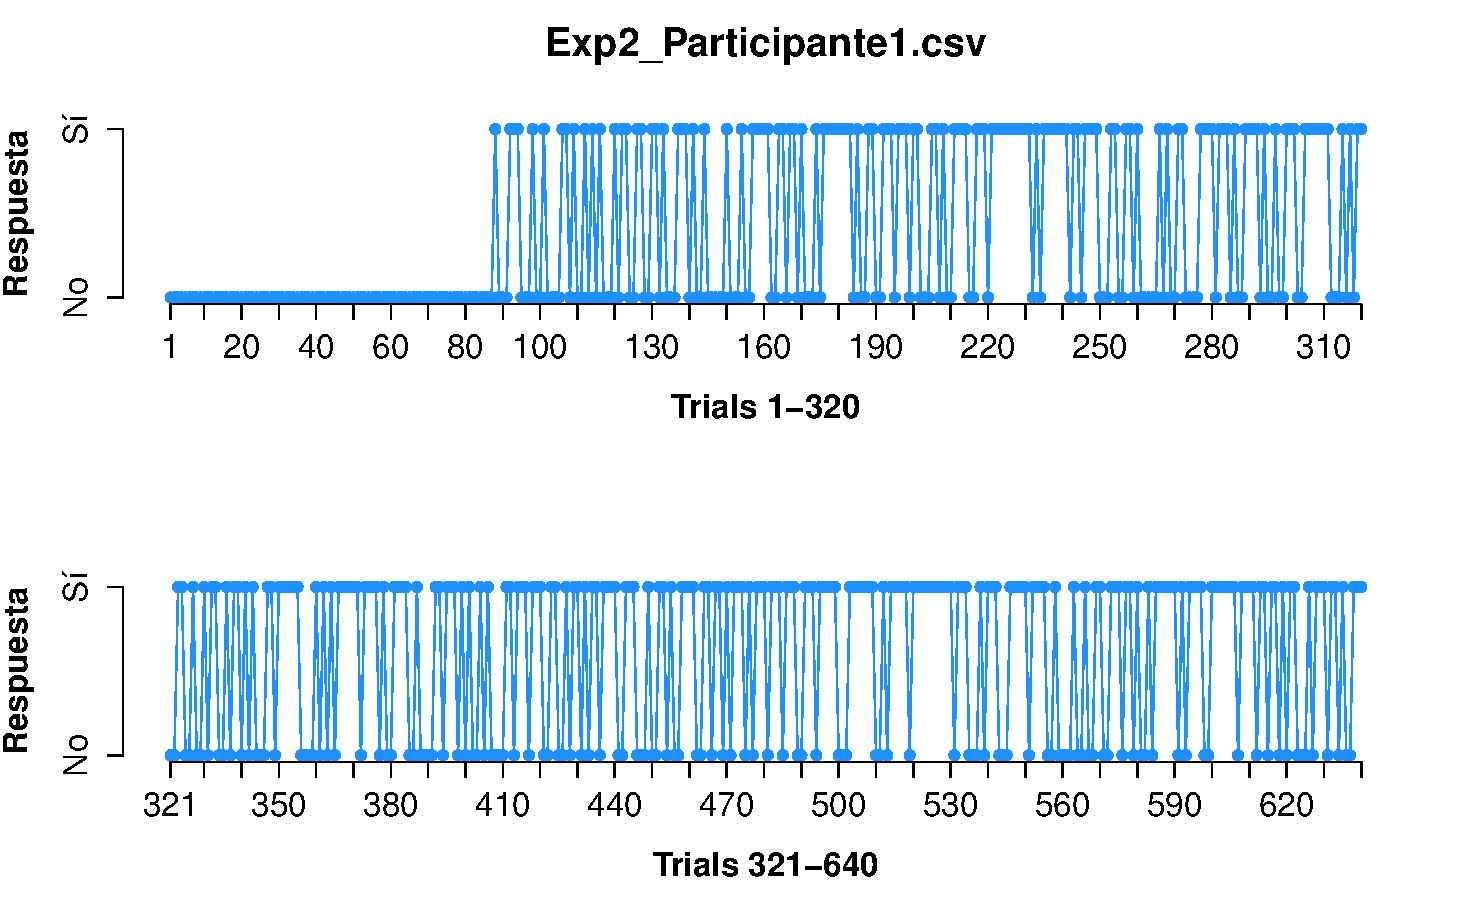
\includegraphics[width=0.60\textwidth]{Figures/Response_Exp2_P1} 
%\decoRule
\caption[Respuesta emitida por ensayo: Ejemplo de participante sesgado]{Se muestran las respuestas "Sí/No" emitidas en cada uno de los 640 ensayos del Experimento 1 por el Participante 1. La gráfica superior muestra los primeros 320 ensayos y la gráfica inferior, los 320 restantes. En el panel superior se aprecia con claridad un tren de respuesta que se extiende a lo largo de 80 ensayos, durante los cuales el Participante 1 sólo utilizó una de las opciones de respuesta posibles.}
\label{fig:Resp_E2_P1}
\end{figure}

%Las gráficas correspondientes al resto de los participantes en los Experimentos 1 y 2, se muestran en las Figuras~\ref{fig:Response_P1} y \ref{fig:Response_E2}, respectivamente.\\

\item Correlación entre las respuestas 'Sí/No' emitidas y el tipo de estímulo presentado en cada ensayo.

A continuación, sobre estas mismas gráficas se añadieron indicadores que señalaran las características específicas de los estímulos presentados en cada ensayo -es decir, si se trataba de una Señal o Ruido y si se trataba de un estímulo Fácil o Difícil-.\\ 

Retomando el caso del Participante 1 del Experimento 2 presentado en la Figura~\ref{fig:Resp_E1_P1}, la Figura~\ref{fig:BiasResp_E1_P1} explora la posibilidad de que las respuestas registradas de hecho estuvieran relacionadas con los estímulos presentados en pantalla, (por ejemplo, en el improbable -pero posible- caso de que se le hubiera presentado una gran proporción de estímulos con Ruido durante los primeros 80 ensayos del experimento). De acuerdo con esta gráfica, parece ser que el tren de 80 respuestas 'No' consecutivas se mantuvo con independencia del tipo de estímulo presentado. Con base en ello, se decidió eliminar a dicho participante de la muestra a analizar, pues se encontró evidencia suficiente para dudar de la atención con que estuvo respondiendo a la tarea.\\

\begin{figure}[th]
\centering
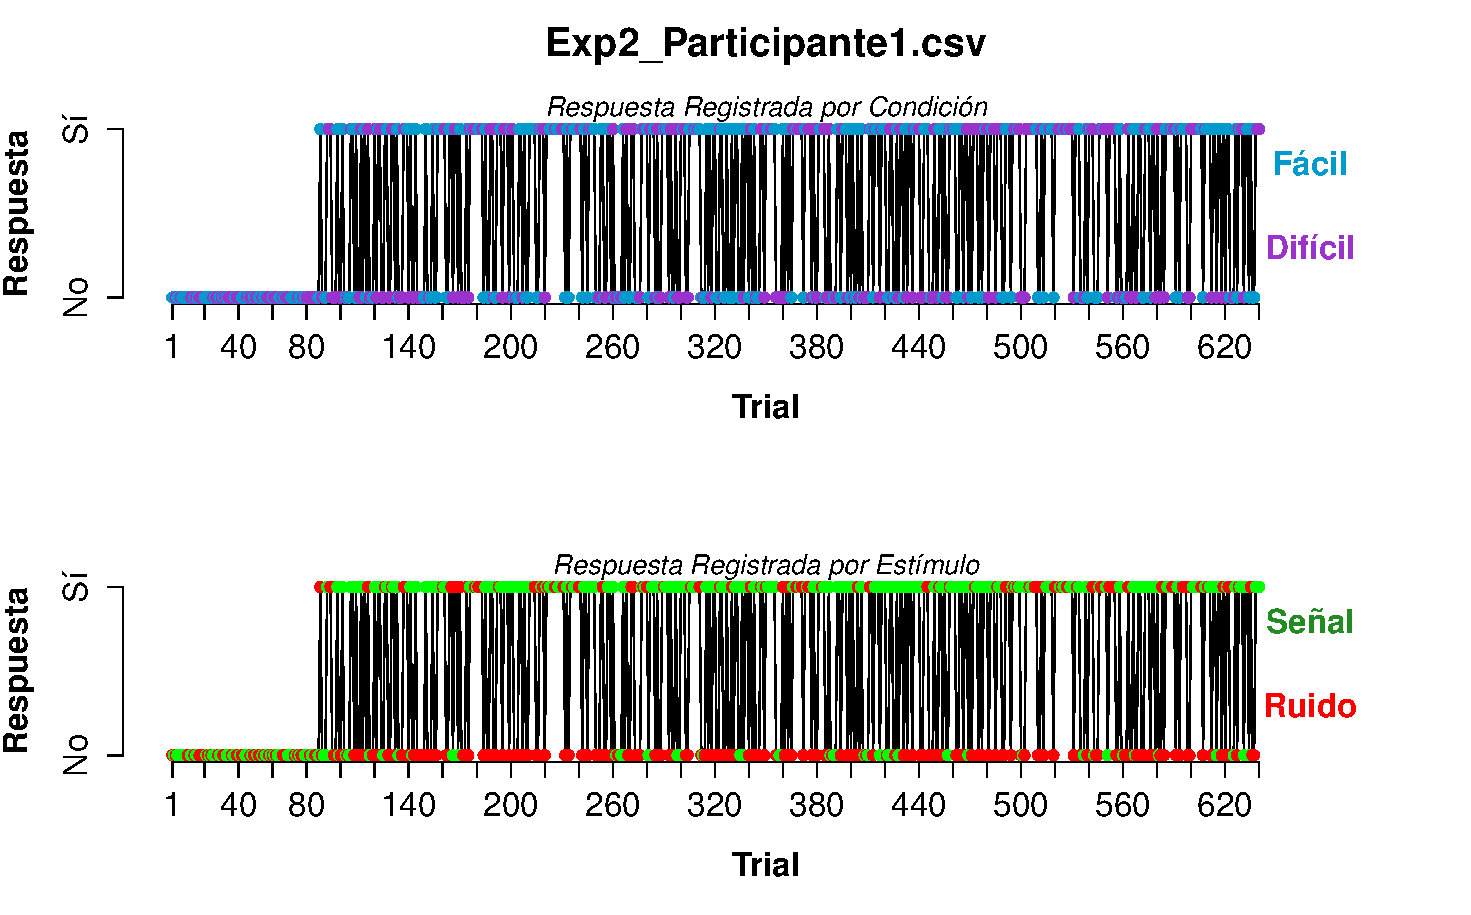
\includegraphics[width=0.60\textwidth]{Figures/BiasResp_Exp2_P1} 
%\decoRule
\caption[Respuesta por Tipo de Estimulo; ejemplo de participante sesgado]{Se muestran las respuestas registradas por el Participante 1 en cada uno de los 640 ensayos del Experimento 2, indicando con diferentes colores el tipo de estímulo que se le mostraba en cada ocasión. En el panel superior se señala con colores violeta y azul si el estímulo presentado pertenecía a la categoría Difícil o Fácil, respectivamente. En el panel inferior se indica si se trataba de una señal o ruido, señalándolos con los colores verde y rojo, respectivamente.}
\label{fig:BiasResp_E1_P1}
\end{figure}

%Las Figuras~\ref{fig:BiasResp_E1} y () muestran las gráficas correspondientes al resto de los participantes en el Experimento 1 y 2, respectivamente.\\

\item Asignación de puntajes de confianza, ('1','2' y '3').

En la segunda fase del problema de detección presentado en cada ensayo, los participantes tenían que elegir entre tres opciones de respuesta (teclas 1, 2 y 3) para señalar qué tanta confianza tenían sobre la respuesta recién emitida ("poco seguro", "más o menos seguro" o "muy seguro", respectivamente). Las respuestas fueron registradas por el programa como parte de una escala mayor (con valores del 1 al 6), que permite diferenciar entre la confianza de haber rechazado correctamente un estímulo con Ruido (e.g. "1, estoy muy seguro de que los círculos eran diferentes") y la confianza de haber identificado correctamente un estímulo con Señal (e.g "6, estoy muy seguro de que los círculos son iguales"), asignando los valores intermedios (3 y 4) a los puntajes asignados para señalar una confianza baja en la respuesta emitida (e.g. "3, poco seguro de que los círculos eran diferentes" y "4, poco seguro de que los círculos eran iguales").\\

Tal y como se hizo con la tarea de detección binaria, se graficaron los puntajes de confianza registrados por los participantes en cada uno de los 640 ensayos que conformaron cada experimento. A manera de ejemplo, la Figura~\ref{fig:Rating_E2_P4} muestra los puntajes emitidos por el Participante 15 del Experimento 2 a lo largo de la tarea. Este participante, de acuerdo con lo que se esperaría encontrar, utiliza hace uso de las tres teclas de respuesta, que son registradas por el programa de acuerdo a su correspondencia con la respuesta dada a la tarea de detección binaria.\\ 
 
\begin{figure}[th]
\centering
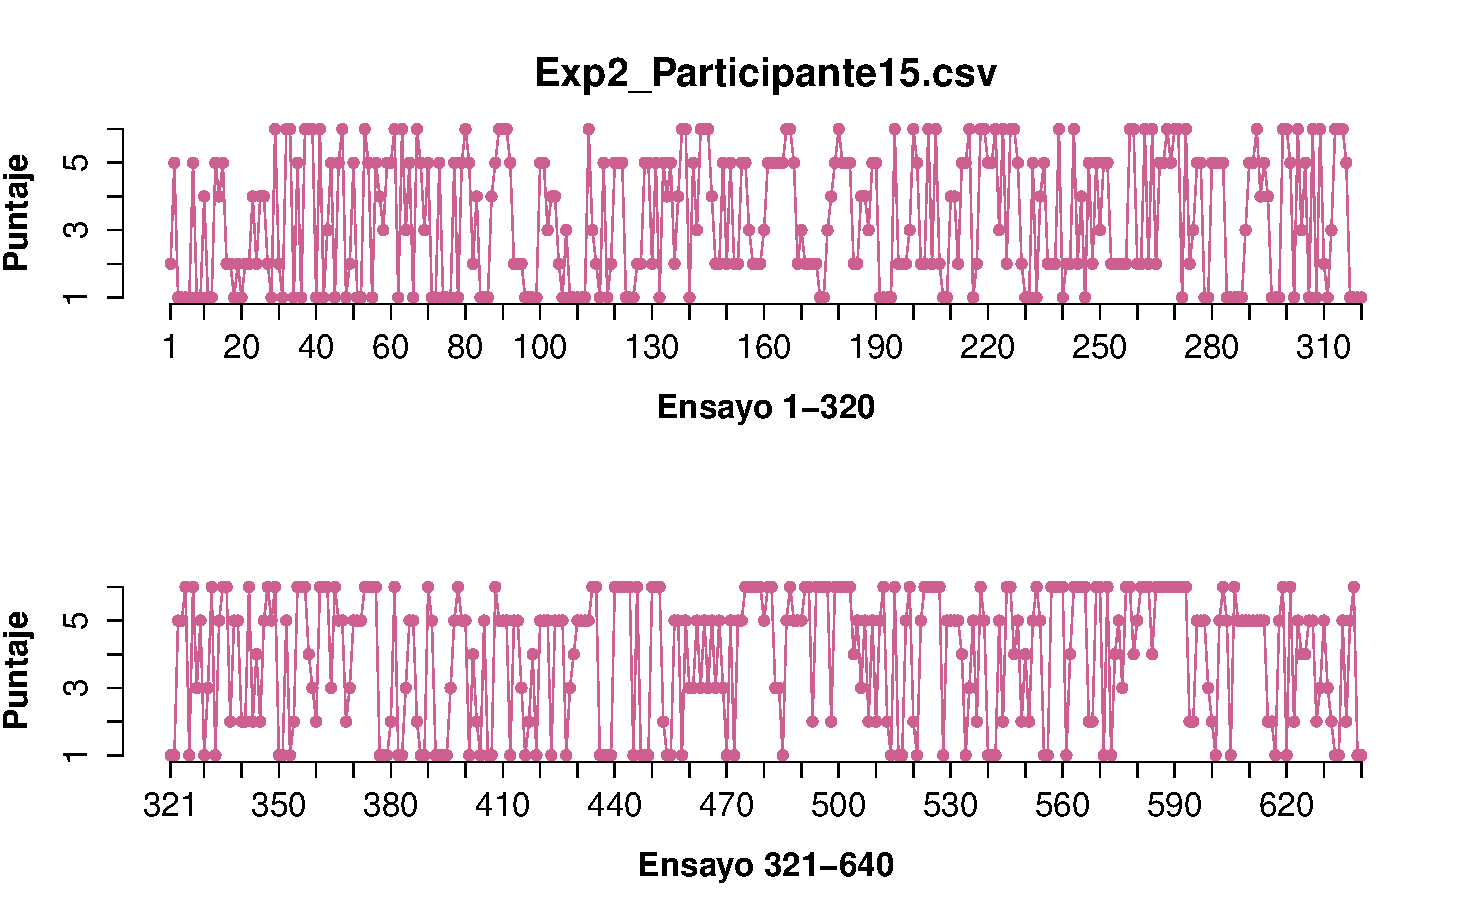
\includegraphics[width=0.60\textwidth]{Figures/Rating_Exp2_P15} 
%\decoRule
\caption[Asignacion Puntaje de confianza: Ejemplo]{Se muestran los puntajes de confianza asignados por el Participante 15 del Experimento 2 a las respuestas emitidas en la tarea binaria, durante cada uno de los 640 ensayos que conforman el experimento. El panel superior muestra los puntajes asignados en los primeros 320 ensayos del experimento; en el panel inferior, los 320 restantes.}
\label{fig:Rating_E2_P4}
\end{figure}

%El registro ensayo a ensayo de los puntajes de confianza asignados por el resto de los participantes en los Experimentos 1 y 2 se muestran en las Figuras~\ref{fig:Rating_E1} y \ref{fig:Rating_E2}, respectivamente.\\

\end{itemize}










\subsection{Control 2: ¿La duración del experimento tuvo un impacto en la ejecución de los participantes?}

La Fatiga causada por la extensión del experimento y la posible Habituación a la ilusión óptica, fueron dos de las fuentes de ruido externo que más preocupación causaron en términos de garantizar la fiabilidad de los datos obtenidos. Para preveer su influencia sobre el desempeño de los participantes, se incluyeron un par de controles en el diseño experimental, tales como una pantalla de espera entre ensayos que daba oportunidad a los participntes de descansar e indicar cuando se sintieran listos para atender un nuevo par de estímulos, o la restricción del tiempo durante el que se mostraban los estímulos a comparar. De cualquier forma, una vez obtenidos los datos correspondientes a la ejecución de los participantes, se realizó un segundo conjunto de gráficas con el objetivo de verificar que el efecto de Fatiga o Habituación no se hayan presentado durante la tarea, como se vería reflejado por un decaimiento o mejora del desempeño de los participantes con el paso del tiempo.\\ 

\begin{itemize}
\item Aciertos y errores a lo largo del tiempo

Primero, se construyeron gráficas que permitieron observar si las respuestas emitidas por los participantes en cada ensayo, fueron registradas como aciertos o errores. Esto se realizó con el objetivo de explorar visualmente la existencia de cambios significativos en el desempeño de los participantes a lo largo del tiempo, conforme adquirían más experiencia en la tarea.\\

La Figura~\ref{fig:Success_E2_P14} muestra como ejemplo, el desempeño del Participante 14 a lo largo del Experimento 2. La gráfica superior presenta el registro acumulativo de los aciertos y errores cometidos a lo largo del experimento. En los paneles inferiores se muestra -ensayo a ensayo- si las respuestas registradas fueron clasificadas como acierto o error, dependiendo su correspondencia con el tipo de ensayo evaluado.\\

\begin{figure}[th]
\centering
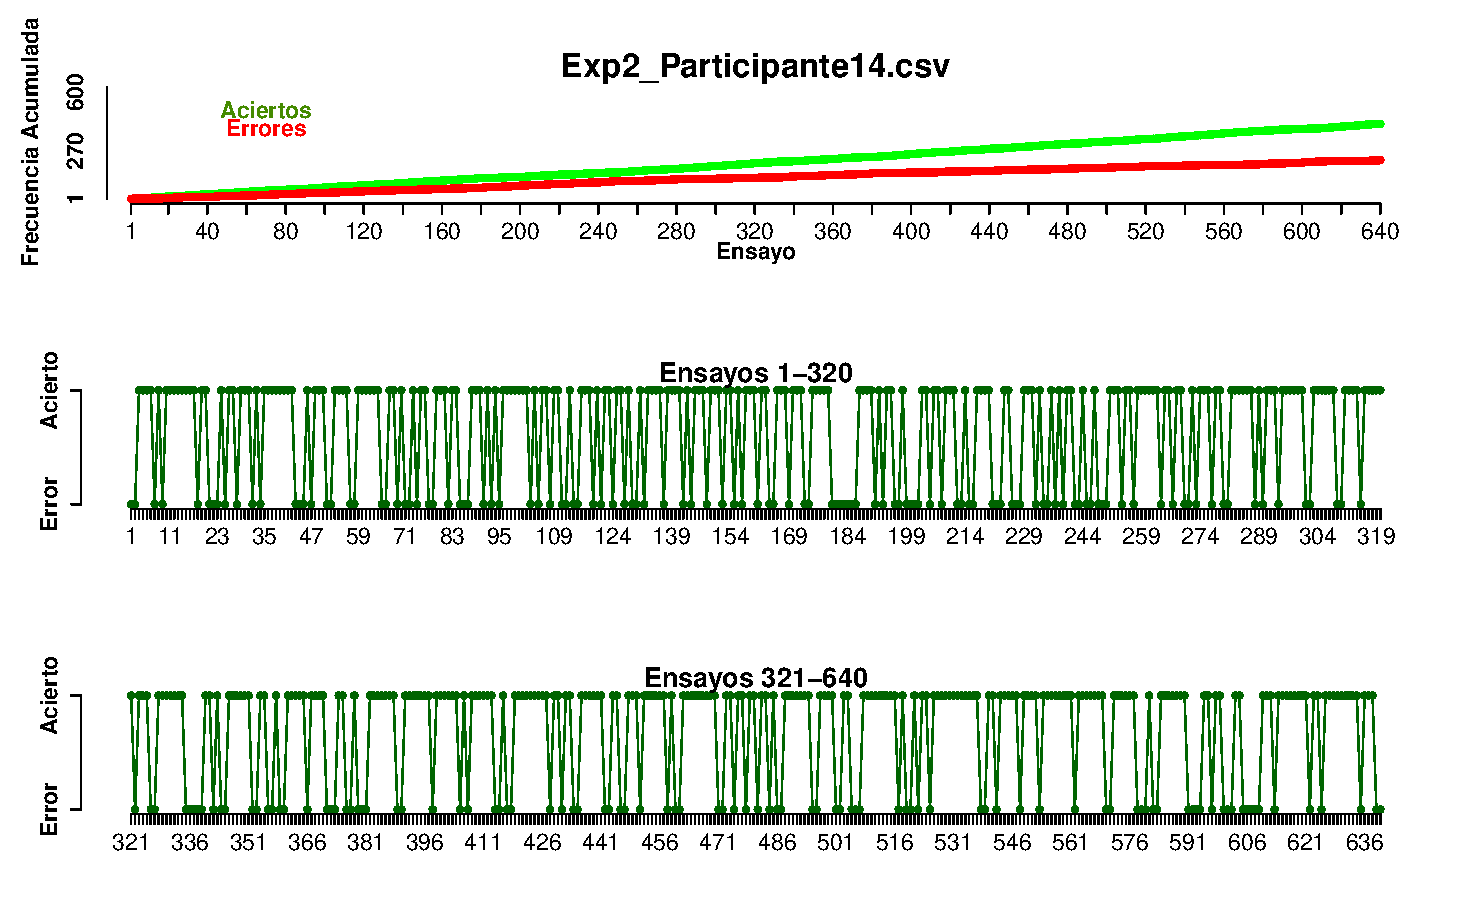
\includegraphics[width=0.60\textwidth]{Figures/Success_Exp2_P14}
%\decoRule
\caption[Aciertos y errores a lo largo del tiempo: Participante ejemplar]{Aciertos y errores cometidos por el Participante 14 del Experimento 2 a lo largo de la tarea. En el panel superior se muestra el registro acumulativo de estos a lo largo del experimento, en tanto que los paneles inferiores muestran la clasificación ensayo a ensayo de las respuestas emitidas por el participante como Acierto o Error, (siendo que el panel intermedio presenta la primera mitad del experimento y el panel inferior, el resto).}
\label{fig:Success_E2_P14}
\end{figure}

%Las Figuras~\ref{fig:Success_E1} y \ref{fig:Success_E2} muestran los aciertos y errores cometidos a lo largo de los experimentos por el resto de los participantes en los Experimentos 1 y 2, respectivamente.\\


\item Resultados a lo largo del tiempo

Además de identificar los aciertos y errores cometidos por los participantes a lo largo de los experimentos, se realizaron también gráficas que señalaran qué tipo de acierto o error habían cometido los participantes en cada ensayo. Nuevamente, se presentan los datos obtenidos de la ejecución del Participante 14 del Experimento 2 en la Figura~\ref{fig:Outcome_E2_P14}, en un par de gráficos donde se señalan los resultados obtenidos a lo largo de la tarea: El panel superior muestra el registro acumulativo de los cuatro posibles resultados a obtener a lo largo del experimento y en el panel inferior se presentan los resultados obtenido en cada ensayo.\\ 

\begin{figure}[th]
\centering
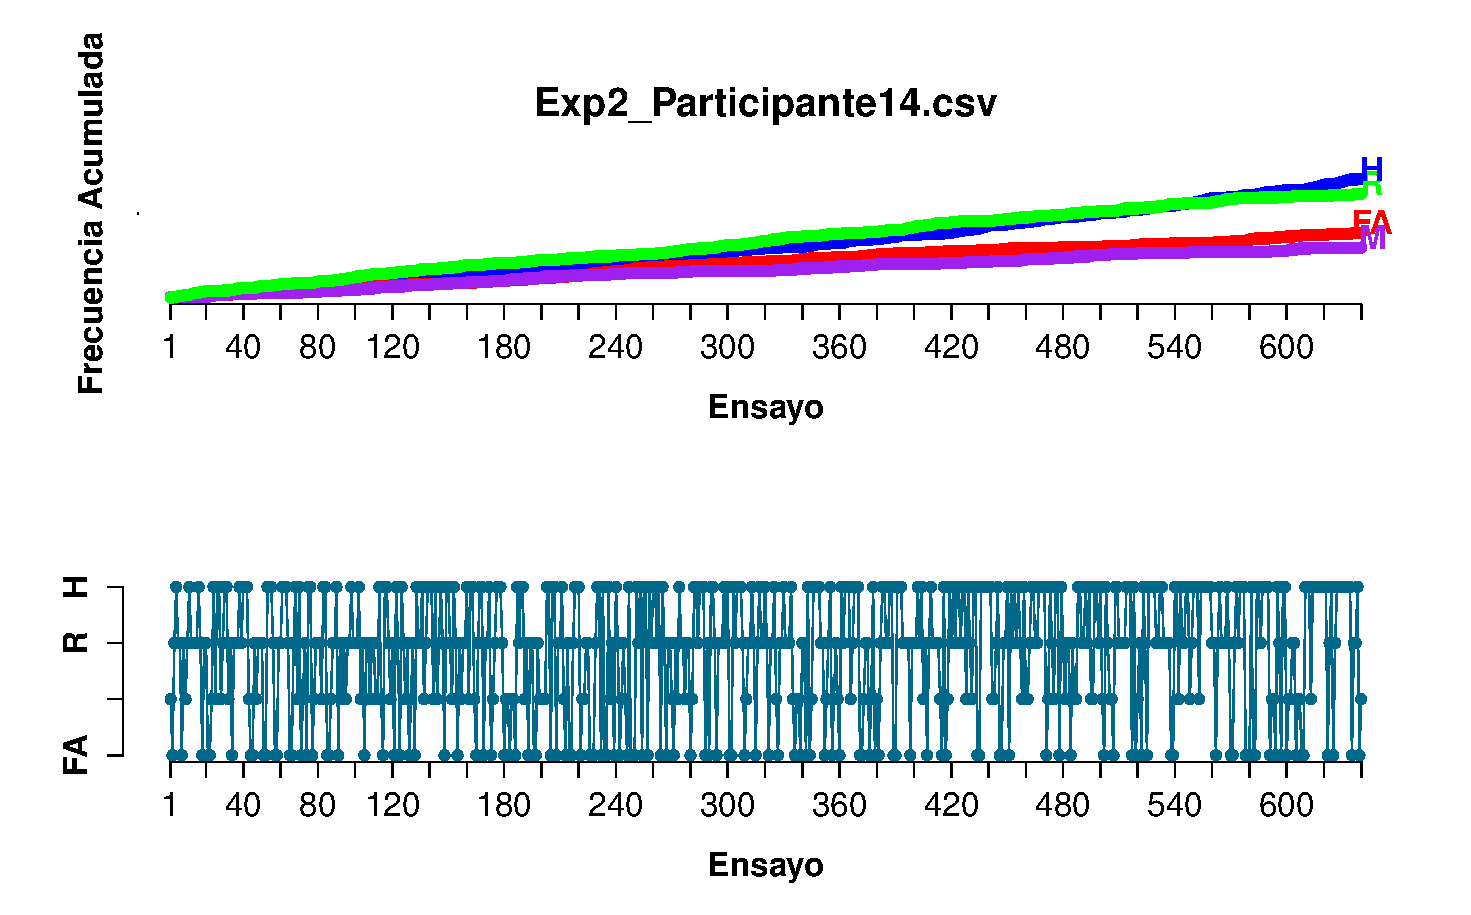
\includegraphics[width=0.60\textwidth]{Figures/Outcome_Exp2_P14}
%\decoRule
\caption[Resultado obtenido a lo largo del tiempo: Ejemplo]{Resultados obtenido por el Participante 14 del Experimento 2 a lo largo del Experimento. En el panel superior se muestra la frecuencia acumulativa de los  Hits, Falsas Alarmas, Rechazos y Omisiones obtenidos durante el experimento, mientras que en el panel inferior se presenta el resultado obtenido en cada uno de los 640 ensayos.}
\label{fig:Outcome_E2_P14}
\end{figure}

%El resto de los participantes en los experimentos 1 y 2 aparecen en las Figuras~\ref{fig:Outcome_E1} y \ref{fig:Outcome_E2}, respectivamente.\\

\end{itemize}










\subsection{Control 3: ¿El diseño de los estímulos afectaron el desempeño de los participantes?}

Durante la construcción de los estímulos a presentar en los experimento se manipuló arbitrariamente la presentación de dos variables: 1) El número de círculos externos incluidos en las figuras de Ebbinghaus y 2) el color en que se presentaron las figuras. La primera constituye la variable experimental, con la que se buscó diseñar las dos condiciones de dificultad entre las que se compararía el desempeño de los participantes. En tanto que en el caso de la segunda, las variaciones en la misma fueron incluidas de manera arbitraria en un intento por hacer de la tarea menos tediosa y más dinámica, buscando preveer los efectos de Fatiga y Habituación.\\

En otras palabras, se esperaba que el desempeño de los participantes variara exclusivamente en función a los cambios en la variable experimental. Para descartar la posibilidad de que el desempeño de los participantes se hubiera visto influido por otro tipo de características en los estímulos presentados (el color en que estos fueron construidos), se realizaron gráficas que permitieran explorar visualmente la posible relación entre el color en que se presentaban las figuras y el desempeño de los participantes.\\

\begin{itemize}
\item El efecto del color sobre la intensidad de la ilusión.

Una primer forma en que el color en que las figuras fueron construidas pudo haber afectado el desempeño de los participantes fue alterando la dificultad de la tarea, mediante la atenuación o intensificación de la ilusión óptica presentada. Para evaluar dicha posibilidad, se construyó un subset de gráficas que presentaban el número de aciertos y errores cometidos por los participantes al registrar respuestas afirmativas (Hits y Falsas Alarmas), por cada color.\\

\begin{figure}[th]
\centering
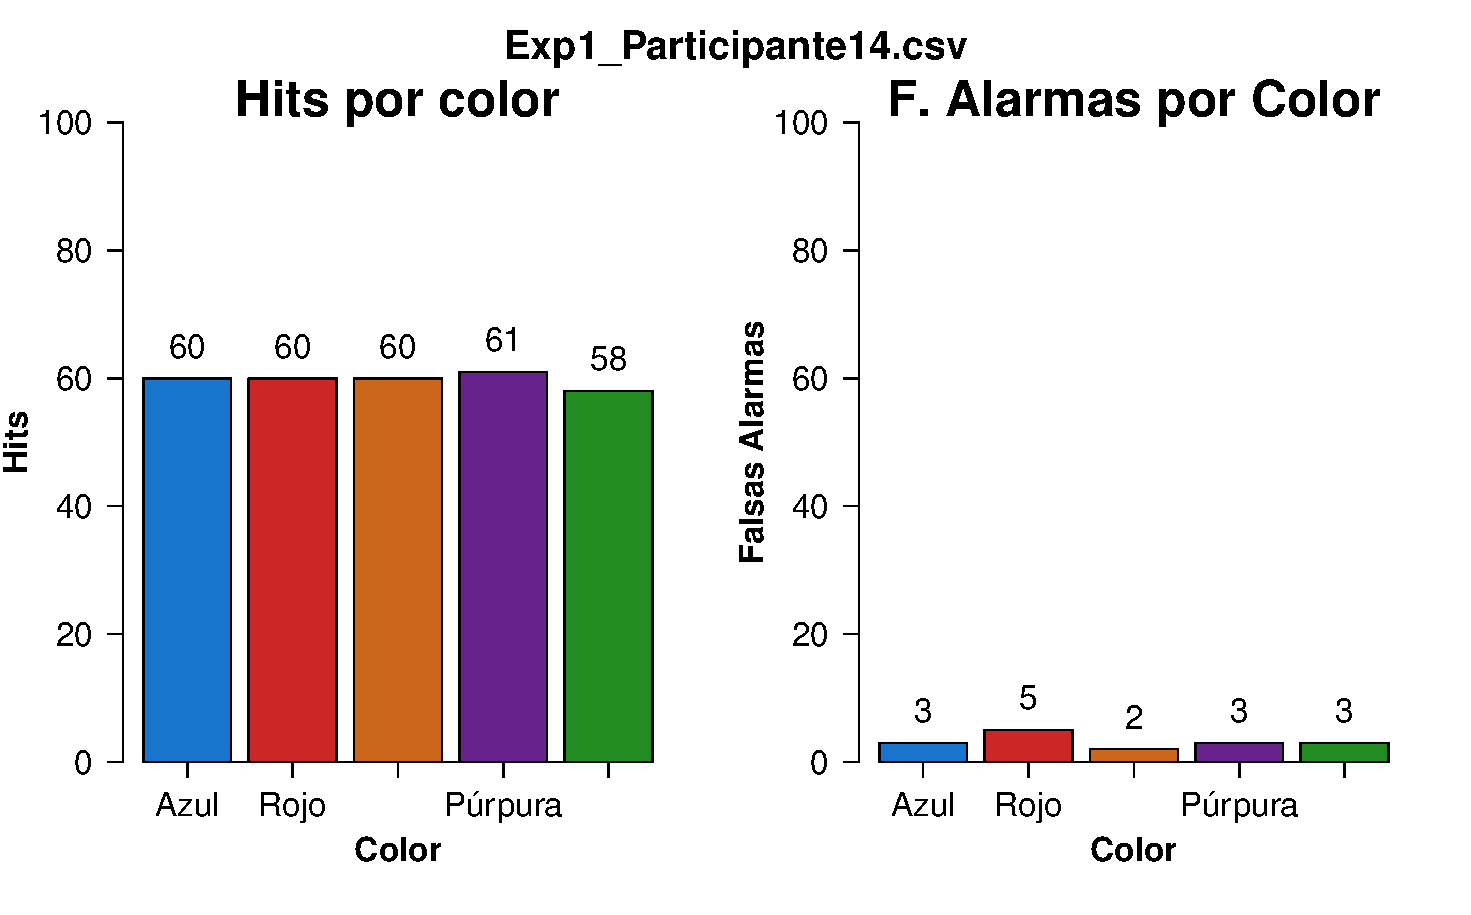
\includegraphics[width=0.60\textwidth]{Figures/Color_Exp1_P14}
%\decoRule
\caption[Hits y Falsas Alarmas por Color; Ejemplo]{Se muestra el desempeño del Participante 14 del Experimento 1 en función del color de los estímulos. En el panel izquierdo se muestra la relación entre el número de Hits obtenidos y el color de los estímulos y en el panel derecho, su relación con las Falsas alarmas. El número de Omisiones y Rechazos Correctos no se incluyen en la figura al tratarse del complemento de los resultados presentados.}
\label{fig:Color_E1_P14}
\end{figure}

Por ejemplo, la Figura~\ref{fig:Color_E1_P14} muestra la cantidad de Hits y Falsas Alarmas cometidas por el Participante 14 a lo largo del Experimento 1 por cada color utilizado en el diseño de las figuras (en el panel izquierdo y derecho, respectivamente). De acuerdo con las gráficas, no parece que el color haya tenido un efecto sobre la precisión con que este participante respondía a la tarea.\\

%Las gráficas correspondientes a la relación entre las frecuencias absolutas de Hits y Falsas Alarmas y el color de los estímulos, para el resto de los participantes en los Experimentos 1 y 2 se encuentran en la Figura~\ref{fig:Color_E1} y \ref{fig:Color_E2}, respectivamente. 

\item El Efecto del Color sobre la emisión de respuestas en los participantes.

Una segunda forma en que el color los estímulos fueron presentados pudo haber alterando el desempeño de los participantes, es si estos hubieran mostrado un sesgo o preferencia a responder de cierta forma ante alguno de los colores utilizados, con independencia del resto de las características de las figuras a evaluar. Para explorar dicha posibilidad, se trazó un último subconjunto de gráficas que mostraran la relación entre el color de las figuras y la proporción de respuestas afirmativas o negativas emitidas por los participantes.\\

La Figura~\ref{fig:BiasCol_E1_P13} presenta un ejemplo de este tipo de gráficas y muestra la proporción de Respuestas "Sí/No" emitidas por el Participante 13 del Experimento 1 para cada uno de los diferentes colores en que se presentaron los estímulos. Como se puede ver en la figura, parece ser que este participante mantuvo constante la proporción de respuestas afirmativas y negativas emitidas a lo largo de los distintos colores utilizados, por lo que no parece que el color esté ejerciendo alguna influencia sobre su manera de responder a los estímulos presentados.\\

\begin{figure}[th]
\centering
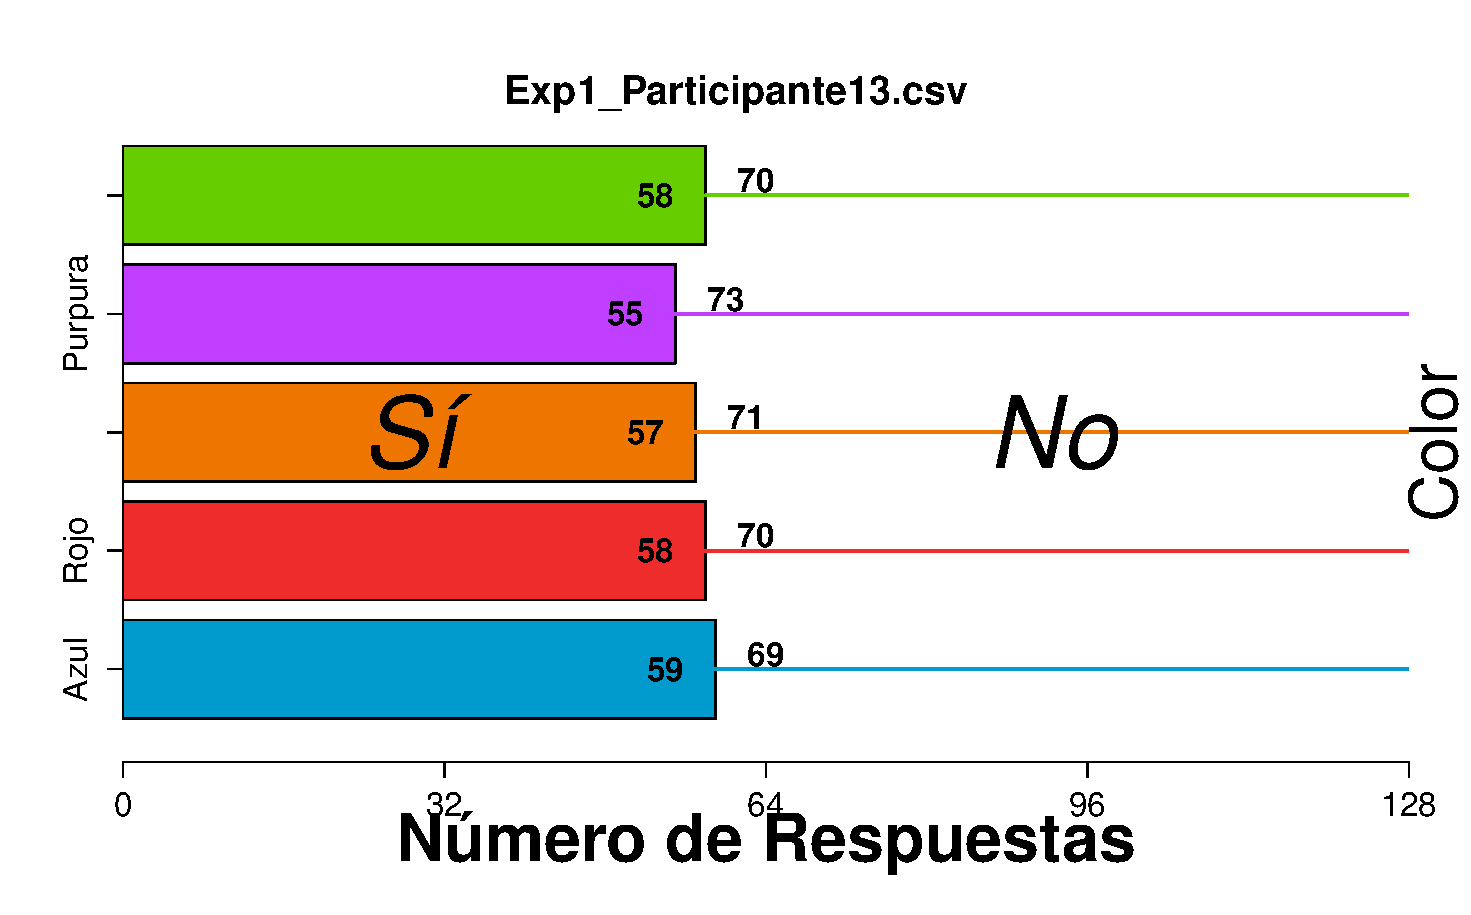
\includegraphics[width=0.40\textwidth]{Figures/BiasColor_Exp1_P13}
%\decoRule
\caption[Proporción de Respuestas "Sí/No" por color; Ejemplo]{Se muestra la proporción de respuestas afirmativas y negativas emitidas por el Participante 14 del Experimento 1, en función al color en que se le presentaban los estímulos.}
\label{fig:BiasCol_E1_P13}
\end{figure}

%Las Figuras~\ref{fig:BiasCol_E1} y ~\ref{fig:BiasColor_E2} muestran las gráficas correspondientes al resto de los participantes en los Experimentos 1 y 2, respectivamente. 

\end{itemize}

En cualquier caso, el número de figuras presentadas en cada color se mantuvo constante entre los tipos de ensayo (Ruido y Señal) y las clases de estímulos (Fácil y Difícil). Es decir, que aún cuando se hubiera encontrado evidencia de variaciones en el desempeño de los participantes en función de los colores utilizados, se esperaría que dicho efecto se distribuyera de manera homogénea entre las dos clases de estímulos entre las cuales se compararía su ejecución.\\

Las gráficas correspondientes al desempeño de cada uno de los participantes en los Experimentos 1 y 2 se presentan el los Apéndices.\\




































\section{Análisis estadísticos}

En cada una de las tareas contenidas en los experimentos realizados (la tarea de detección binaria y el procedimiento de escala de confianza), los patrones de respuesta identificados como parte del Efecto Espejo se presentaron en al menos tres cuartas partes de los participantes. De los veinte participantes en el Experimento 1, diecisiete ($85\%$) mostraron el patrón de respuesta esperado en la tarea binaria y dieciocho ($90\%$) en la escala de confianza. A su vez, en el Experimento 2, dieciocho de los veinte participantes incluidos en la muestra ($90\%$) presentaron el mismo patrón en ambas tareas. Estas proporciones resultan estadísticamente significativas al compararlas contra el azar con una prueba binomial ($p=0.0025$ y $p=0.0004$ en el caso de las proporciones reportadas en el Experimento 1, respectivamente, y $p=0.0004$ para lo reportado en el Experimento 2).\\

Tomando en cuenta que el diseño de las clases de estímulos a comparar se realizó de manera exploratoria y que los experimentos realizados estuvieron compuestos por una tarea de detección que se presentó en términos de dos sub-tareas, el análisis de los datos recabados se llevó a cabo en el siguiente orden:\\

\begin{enumerate}
\item \textbf{Verificar que realmente existiera una diferencia entre las clases de estímulos construidas}\\

Dado que los niveles de dificultad propuestos fueron construidos con base en la literatura revisada en el funcionamiento de la ilusión de Ebbinghaus, un primer punto a tratar en materia del análisis de los datos obtenidos estuvo orientado a evaluar si las clases de estímulos creadas realmente diferían en términos de su discriminabilidad. Para ello, se compararon los valores de $d'$ calculados a partir de los subconjuntos de Hits y Falsas Alarmas obtenidos por cada condición, para evaluar que se cumpliera la siguiente relación:\\

\begin{center}
 $d'(A) > d'(B)$\\
 donde A y B representan los dos niveles de dificultad construidos para las tareas en función del número de círculos externos contenidos en las tareas: la clase de estímulos A con "pocos círculos" (2 o 3 círculos) y la clase B con "muchos círculos" (7 u 8 círculos)\\
\end{center}

\item \textbf{Comparar las tasas de Hits y Falsas Alarmas entre condiciones.}\\

Una vez corroborada la diferencia entre las clases de estímulos construidas, se evaluó que las diferencias entre la discriminabilidad asociada a cada clase de estímulos se reflejaran tanto en el número de aciertos como en el número de errores cometidos en la tarea de respuestas binarias, como se reporta en la literatura en Memoria de Reconocimiento a partir del siguiente patrón de respuesta:\\

\begin{center}
$H(A) > H(B)$\\
$FA(B) > FA(A)$\\
donde $H$ y $FA$ representan las tasas de Hits y Falsas Alarmas obtenidas en cada clase de estímulo a evaluar. Es decir:\\
$FA(A) < FA(B) < H(B) < H(A)$\\
\end{center}

\item \textbf{Comparar el puntaje de confianza promedio asignado a cada tipo de ensayo entre los niveles de dificultad.}\\

Posteriormente, se compararon los puntajes de confianza asignados a cada tipo de ensayo (Señal o Ruido) por cada clase de estímulo (Fácil o Difícil).\\

Primero, en función de los puntajes de confianza crudos asignados por los participantes -el registro de las teclas de respuesta 1, 2 y 3-, se esperaba encontrar la siguiente relación en función de los niveles de dificultad:

\begin{center}
$P(A) > P(B)$\\
donde $P$ refiere al promedio de los puntajes de confianza asignados a las respuestas emitidas por los participantes durante la tarea binaria, por cada condición de dificultad.\\
\end{center}

Después, tomando en cuenta que los experimentos fueron programados de tal manera que los puntajes registrados por los participantes -para indicar qué tan seguros se sentían respecto de la respuesta emitida en ese mismo ensayo a la tarea de detección binomial- fueran "transformados" a valores dentro de una escala mayor que distingue entre la confianza en las respuestas negativas y la confianza en las respuestas afirmativas, se espera encontrar la misma relación reportada en Memoria de Reconocimiento entre los promedios de los puntajes de confianza asignados por cada tipo y clase de estímulos:\\

\begin{center}
$P(AS) > P(BS)$\\
$P(AN) < P(BN)$\\
donde nuevamente $P$ refiere al promedio de los puntajes de confianza asignados a cada tipo de ensayo por cada clase de estímulo. Es decir:\\
$P(AN) < P(BN) < P(BS) < P(AS)$\\
\end{center}

\item \textbf{Réplica de controles reportados en la literatura.}\\

Además de la evaluación de las diferencias encontradas en la ejecución de los participantes a través de las clases de estímulos construidas, en la literatura que reporta evidencia del Efecto Espejo en estudios de Memoria de Reconocimiento se reportan también algunos controles adicionales en el análisis de datos para confirmar la solidez del Efecto Espejo encontrado en los mismos, \parencite{Glanzer1990}. En el presente trabajo se incorpó uno de dichos controles y se revisó la posible correlación entre los tiempos de respuesta y los niveles de dificultad construidos. De acuerdo con la literatura, descartar esta correlación en particular permite afirmar que las diferencias halladas en el desempeño de los participantes están ligadas a la discriminabilidad entre los estímulos con Señal y Ruido que componen cada clase y por el contrario, no pueden ser explicados como un reflejo de qué tanto tiempo dedicaron los participantes a decidir sus respuestas en cada nivel de dificultad.\\
\end{enumerate}

Todos los análisis previamente descritos fueron realizados desde dos enfoques distintos:\\

\begin{itemize}
\item Como una réplica de los análisis reportados en la literatura. \textit{(ANOVA's y Pruebas T)}.\\

Tomando en cuenta que el objetivo princial del trabajo de investigación realizado fue evaluar la generalizabilidad de los patrones de respuesta identificados en Memoria de Reconocimiento como Efecto Espejo en una tarea de detección perceptual, se consideró necesario someter los datos obtenidos a los mismos procesos de análisis reportados en la literatura. Para ello, se utilizó como guía un artículo donde se reporta evidencia del Efecto Espejo en cinco experimentos en Memoria de Reconocimiento que manipulan distintas variables para la definición de las clases de estímulos A y B, \parencite{Glanzer1990}. El anális de datos aquí presentado fue realizado con una copia de dicho artículo en mano.\\ 

\item El desarrollo de modelos Bayesianos para la estimación paramétrica y la evaluación de la evidencia encontrada.\\

La estadística bayesiana constituye una herramienta flexible para el análisis de datos, pues se sostiene sobre la base de un conjunto sólido de axiomas que permiten formalizar y evaluar las creencias que se tienen sobre el funcionamiento de ciertos procesos psicológicos -las hipótesis del investigador-, a partir de la especificación de las distribuciones prior y funciones de verosimilitud que describen la relación entre los datos obtenidos sobre el desempeño de los participantes y los modelos estadísticos-cognitivos desarrollados que pretenden dar cuenta de los procesos psicológicos que subyacen a su generación, \parencite{Lee2011}.\\

En el presente trabajo de tesis, además de realizar los análisis de estadística frecuentista correspondientes a la réplica de los estudios reportados en Memoria de Reconocimiento, se incluyeron análisis y modelos bayesianos que permitieran ahondar con mayor detalle en la variabilidad contenida en las respuestas emitidas por los participantes.\\
\end{itemize}










\subsection{Evaluación de las diferencias entre las clases de estímulos propuestas}


Como se mencionó en el capítulo anterior, el Efecto Espejo ha sido reportado en estudios en Memoria de Reconocimiento donde se compara el desempeño de los participantes entre dos clases de estímulos A y B que difieren en la precisión con que sus elementos son reconocidos al presentarse en más de una ocasión. En el caso de las tareas de detección perceptual diseñadas como parte del presente trabajo de tesis, los niveles de dificultad propuestos fueron construidos con base en los efectos que se ha reportado que tienen ciertas variables sobre la intensidad de la ilusión óptica evocada por la figura de Ebbinghaus, \parencite{Massaro1971}. De acuerdo con estos estudios, se propusieron las siguientes dos clases de estímulos:\\

\begin{itemize}
\item Clase A (Fácil)\\

Figuras de Ebbinghaus compuestas por 2 o 3 círculos externos.\\

\item Clase B (Difícil)\\

Figuras de Ebbinghaus con 7 u 8 círculos externos.\\
\end{itemize}

Para evaluar la eficacia del diseño de las clases de estímulos propuestas, comprobando que estas realmente difirieron en términos de qué tan difícil resultó para los participantes discriminar entre los estímulos con Señal y aquellos con Ruido, se compararon los valores de $d'$ estimados para cada una de ellas, de acuerdo con el registro de Hits y Falsas Alarmas obtenidos por todos los participantes en los experimentos realizados.\\

\begin{figure}[th]
\centering
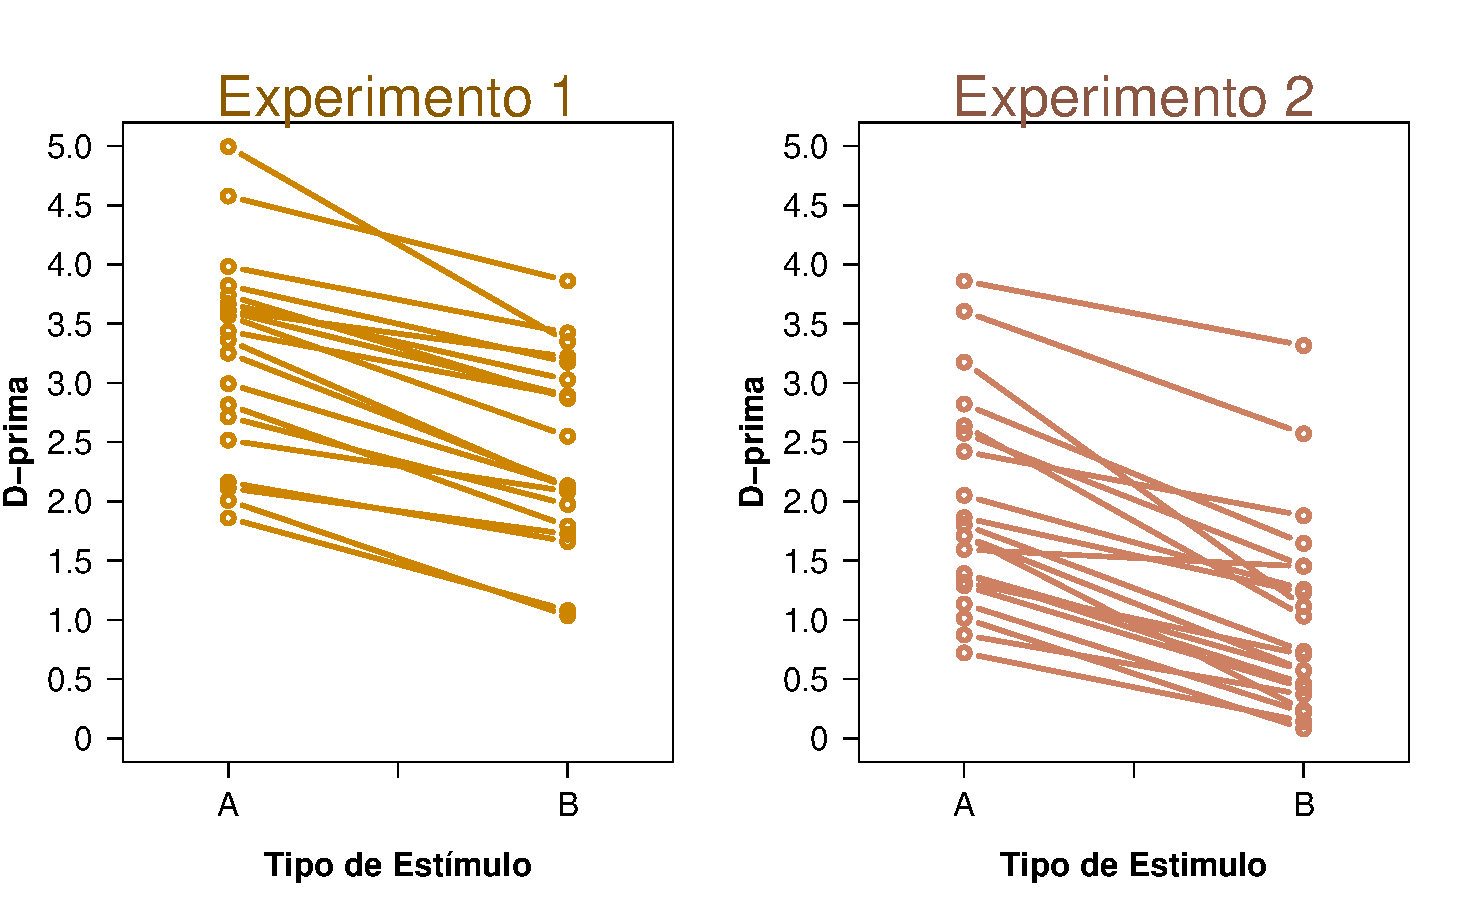
\includegraphics[width=0.90\textwidth]{Figures/Diff_D_E1yE2}
%\decoRule
\caption[Diferencias entre las $d'$ de los niveles de dificultad propuestos]{Por cada uno de los experimentos realizados se muestra la relación entre las d' de cada condición de acuerdo a la ejecución de cada uno de los sujetos. En ambos experimentos, se observa una tendencia sistemática a tener mayores niveles de d' en la condición con pocos círculos en las figuras de Ebbinghaus.}
\label{fig:Diff_D}
\end{figure}

La Figura~\ref{fig:Diff_D} presenta de manera gráfica la comparación entre los valores de $d'$ estimados por cada nivel de dificultad de acuerdo con los datos obtenidos en los Experimentos 1 y 2, relacionando con una línea los pares de $d'$ estimados por cada participante ($d'(A) y d'(B)$). De acuerdo con esta figura, parece ser claro que las clases de estímulos propuestas cumplieron su objetivo, en tanto que puede apreciarse consistentemente la misma tendencia entre participantes a presentar valores mayores de $d'$ en la clase A que en la clase B.\\

A continuación se presentan los análisis realizados para determinar si las discrepancias que parecieran ser evidentes en la Figura~\ref{fig:Diff_D}, son estadísticamente significativas.\\

\textbf{Análisis Frecuentista: Prueba T para comparar las medias de $d'$ por nivel de dificultad}\\

Tal y como se reporta en la literatura, se realizó una prueba T para comparar la precisión con que los participantes podían discriminar los estímulos con Señal y los estímulos con Ruido en cada una de las clases de estímulos construidas. Para ello, se computaron los valores de $d'$ correspondientes al desempeño de los participantes en cada nivel de dificultad y se comparó la diferencia entre los promedios de los valores obtenidos.\\

La Tabla~\ref{Tabla_t-Dprimas} presenta el promedio de las $d'$ computadas por cada nivel de dificultad en cada uno de los experimentos realizados, la diferencia en estas y un indicador sobre su significancia estadística. Como se puede apreciar, la diferencia entre las medias de $d'$ estimadas es significativa en ambos experimentos.\\

\begin{table}
\caption[Prueba T para evaluar las diferencias entre las medias de $d'$ por nivel de dificultad]{Prueba T para evaluar las diferencias entre las medias de $d'$ computadas por nivel de dificultad}
\label{Tabla_t-Dprimas}
\centering
\begin{tabular}{l | c c c c}
\toprule
%\tabhead{Groups} & \tabhead{Treatment X} & \tabhead{Treatment Y} \\
\textbf{Experimento} & \textbf{$\mu d'(A)$} & \textbf{$\mu d'(B)$} & \textbf{T}  & \textbf{P value}\\
\midrule
Experimento 1 & 3.240 & 2.448 & -3.0587 & 0.0020 \\
Experimento 2 & 1.981 & 1.038 & -3.4131 & 0.0007 \\
\bottomrule
\end{tabular}
\end{table}


\textbf{Análisis Bayesiano: Modelo jerárquico bayesiano para evaluar las diferencias en $d'$}\\

Partiendo del modelo bayesiano estándar que describe los supuestos realizados por la TDS, \parencite{LeeBook}, se desarrolló un modelo jerárquico bayesiano (identificado dentro del presente trabajo como Modelo Delta), que asume que tanto los valores de $d'$, como el sesgo $c$ estimado por cada nivel de dificultad se distribuyen de acuerdo a una distribución normal, de donde se extraen los valores computados por cada participante. Bajo este supuesto, el modelo utiliza las inferencias realizadas sobre los valores de $d'$ y $c$ que subyacen al desempeño de cada sujeto para estimar los parámetros que definen la distribución normal de donde se asume que éstos son extraidos (la media ($\mu$) y la desviación estándar $\sigma$). Finalmente, el modelo incorpora un parámetro $\delta$ que computa la diferencias entre las medias de las $d'$ estimadas por concidión.\\

El modelo gráfico que presenta los parámetros y relaciones definidas en el modelo desarrollado se presenta en la Figura~\ref{fig:Mod_Delta} y está compuesto por los siguientes elementos:\\

\begin{itemize}
\item \textbf{Nodos sombreados que representan los datos.}\\

En los modelos gráficos, los nodos representan las variables que el modelo a representar asume tienen una influencia sobre el proceso cognitivo de interés. Dependiendo cómo estén dibujados, los nodos proporcionan información sobre la naturaleza de dichas variables en torno a tres grandes puntos: 1) la variable adopta valores contínuos (nodo circular) o discretos (nodo cuadrado); 2) el valor de la variable es conocido (nodo sombreado) o necesita ser inferido a partir de los datos (nodo claro), y 3) la variable es probabilística (nodo simple) si está determinada por el valor inferido de otras variables (doble nodo), \parencite{LeeBook}.\\

En el caso de nuestros experimentos, los datos registrados de manera directa -a partir de los cuales se desarrolla todo el análisis- son el número de ensayos con Ruido ($n$) y Señal ($s$), y los resultados obtenidos en la tarea: el número total de Hits ($H_ij$) y Falsas Alarmas (($Fa_ij$) cometidos por cada participante ($i$) en cada condición ($j$).\\

\item \textbf{Las tasas de Hits y Falsas Alarmas como una probabilidad oculta.}\\ 

Mientras que en la literatura clásica en TDS las tasas registradas de Hits y Falsas Alarmas son interpretadas como reflejo directo del área de las distribuciones de Señal y Ruido que caen por encima del criterio de elección, \parencite{Wickens, Gescheider, Stainslaw1999}, bajoe el marco del modelamiento bayesiano, el total registrado de Hits y Falsas Alarmas ($H_ij$ y $Fa_ij$) se toma una instancia de un conteo de casos específicos encontrados dentro de un conjunto de observaciones ($s$ y $n$, respectivamente) con cierta probabilidad ($\theta^H_{ij}$ y $\theta^F_{ij}$).\\

En otras palabras, el modelo bayesiano propuesto asume que $H_ij$ y $Fa_ij$ representan un "número de éxitos" extraídos con una probabilidad oculta de un conjunto definido de observaciones, de acuerdo a una distribución binomial con parámetros $p=$ ($\theta^H_{ij}$ o $\theta^F_{ij}$) y $n=$ ($s$ o $n$). Es decir:\\

\begin{center}
$H_{ij}\sim \mathrm{Binomial}\bigl(\theta^H_{ij}, s)$
y
$F_{ij}\sim \mathrm{Binomial}\bigl(\theta^F_{ij}, n)$\\
\end{center}

\item \textbf{Sesgo y Discriminabilidad}\\

De acuerdo con la TDS, la probabilidad que determina las tasas registradas de Hits y Falsas Alarmas ($\theta^H_{ij}$ y $\theta^F_{ij}$) representan el área de las distribuciones de Señal y Ruido que caen por encima de los criterios de elección utilizados por los participantes. Es decir, que dicha probabilidad está definida como la función de densidad acumulada (CDF, por sus siglas en inglés, típicamente representada con el parámetro $\phi$) en una distribución normal estándar para la ubicación de $x$ que corresponde a la diferencia entre $\frac{1}{2}D_{ij}$ (en el caso de los Hits) o $\frac{1}{2}D_{ij}$ (en el caso de las Falsas Alarmas), y la medida de sesgo $C_{ij}$. Es decir:\\

\begin{center}
$\theta^H_{ij}\gets \phi (\frac{1}{2}D_{ij}-C_{ij})$
y
$\theta^F_{ij}\gets \phi (-\frac{1}{2}D_{ij}-C_{ij})$\\
\end{center}

\CONSIDERAR \AGREGAR \UNA \FIGURA \ILUSTRATIVA

\item \textbf{Plato de participantes}\\

En los modelos gráficos bayesianos se utilizan platos para representar lo que en cualquier lenguaje de programación se conoce como un \textit{ciclo for}, \parencite{LeeBook}. Es decir, los platos delimitan conjuntos de parámetros cuyo cómputo se realizará tantas veces como casos -o conjuntos de datos- represente el plato. Por ejemplo, un plato $a$ que contiene los parámetros $p_1, p_2... p_n$ indica que el cómputo de estos se realizará por cada caso contenido en $a$.\\

En el caso del modelo desarrollado, el primer plato ($i$ $participantes$) señala que el cómputo de las probabilidades ocultas tras la emisión de cada par de Hits y Falsas Alarmas registrado ($\theta^H_{ij}$ y $\theta^F_{ij}$) y la estimación del valor de los parámetros $D_{ij}$ y $C_{ij}$ que mejor permitan dar cuenta de dichas probabilidades a partir de la CDF de un par de distribuciones normales, se va a repetir y realizar por cada uno de los participantes ($i$) incluidos en el experimento -es decir, por cada par de Hits y Falsas Alarmas recolectado-.\\

No hay necesidad de incluir los parámetros $n$ y $s$, que representan el total de ensayos con Ruido y Señal contenidos en el experimento, ya que estos permanecen constantes para todos los participantes ($i$) y para todas las clases de estímulos ($j$).\\

\item \textbf{Estructura jerárquica: Distribuciones normales que describen los datos individuales}\\

Como ya se mencionó, la cualidad esencial del modelo desarrollado es que asume que los parámetros $D_{j}$ y $C_{j}$ computados por cada sujeto $i$ provienen de distribuciones normales que describen la discriminabilidad ($d'$) y el sesgo en las respuestas ($c$) asociado a cada clase de estímulos $j$. Dichas distribuciones están definidas por los parámetros $\mu^D_{j}$, $\mu^C_{j}$ y $\sigma^D_{j}$, $\sigma^C_{j}$, que el modelo infiere a partir de los datos ($H_ij$ y $Fa_ij$). Es decir:\\

\begin{center}
$D_{ij}\sim \mathrm{Gaussian}\bigl(\mu^D_{j},\lambda^D_{j})$\\
y\\
$C_{ij}\sim \mathrm{Gaussian}\bigl(\mu^C_{j},\lambda^C_{j})$\\
\end{center}

\item \textbf{Plato de Condición}\\

Un segundo plato ($j$ $condiciones$) señala que el cómputo de los parámetros que definen las distribuciones normales asociadas al sesgo y la discriminabilidad, se va a realizar de manera independiente para cada clase de estímulo, a partir del par de Hits y Falsas Alarmas registrado para cada uno por cada participante ($plato$ $i$ $participantes$).\\

\item \textbf{Parámetro Delta}\\

Finalmente, se incluye un parámetro Delta ($\delta$) que computa directamente la diferencia entre las inferencias realizadas acerca del valor de las medias de $d'$ por cada nivel de dificultad, ($\mu^D_{A}$ y $\mu^D_{B}$). Es decir:\\

\begin{center}
$\delta \gets \mu^D_{A}-\mu^D_{B}$\\
\end{center}

El parámetro $\delta$ está representado con un doble nodo para señalar que es un parámetro determinado por los valores estimados para otras variables ($\mu^D_{A}$ y $\mu^D_{B}$) de manera directa -no probabilística-.\\
\end{itemize} 


\begin{figure}[th]
\centering
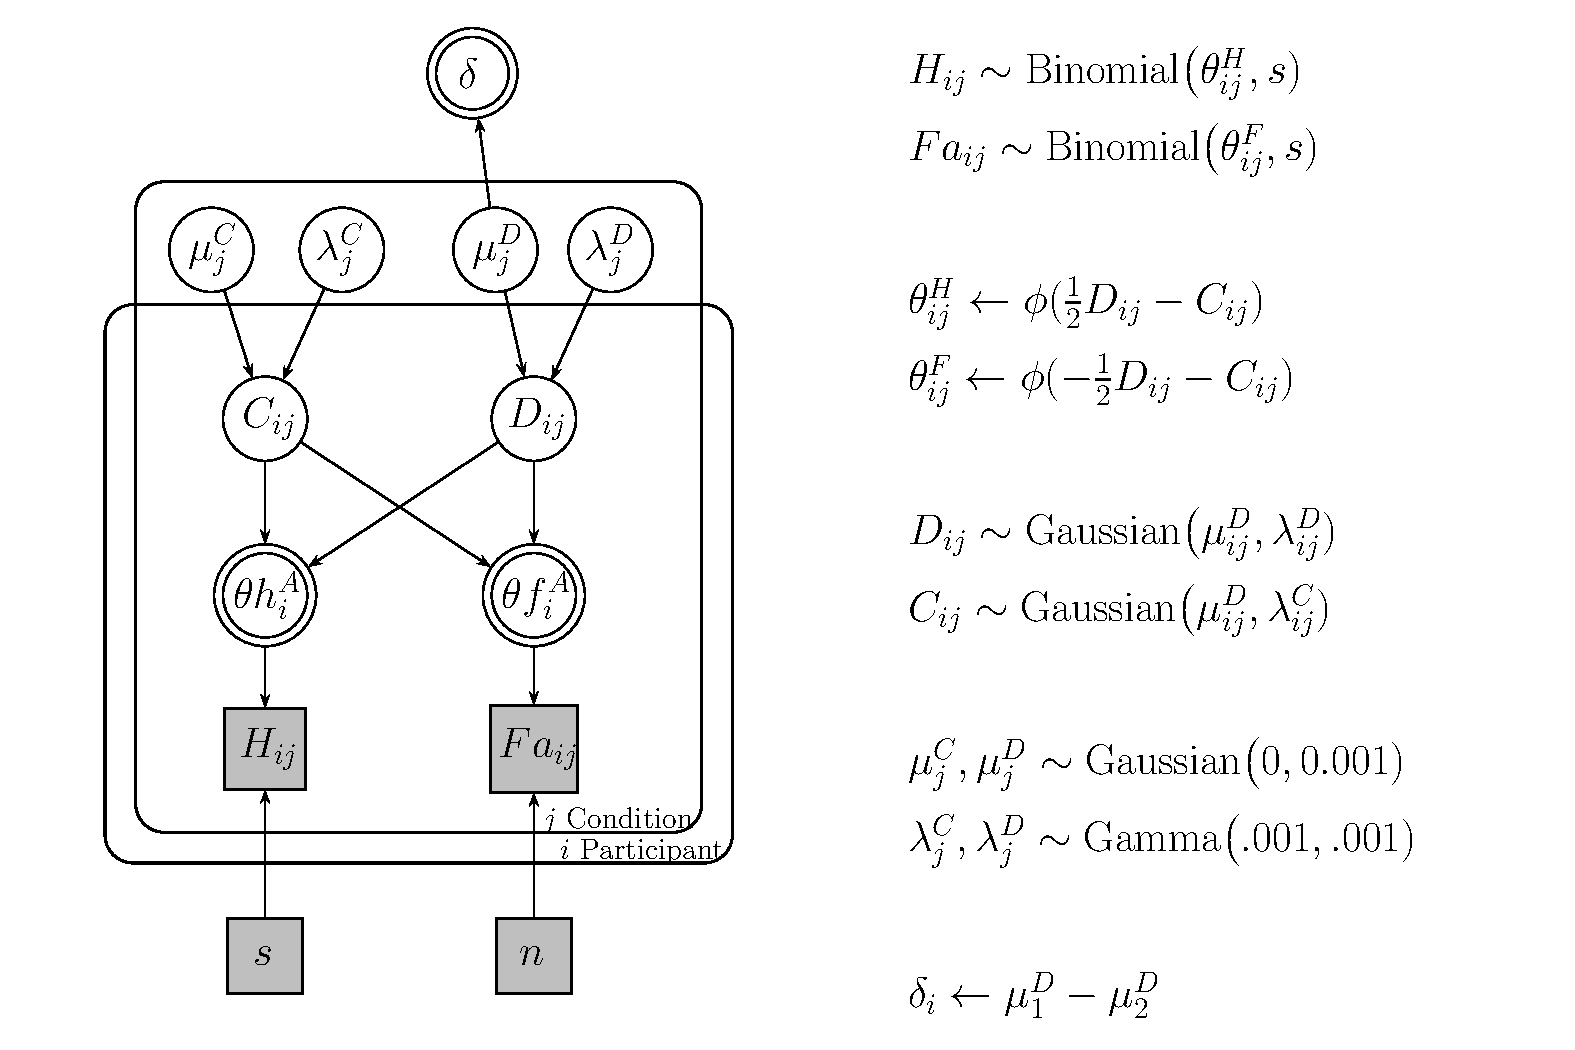
\includegraphics[width=1.1\textwidth]{Figures/Model_Delta_Diff_D}
%\decoRule
\caption[Modelo Delta: Modelo jerárquico bayesiano para revisar las diferencias en $d'$ entre clases de estímulos]{Modelo jerárquico bayesiano que asume que la $d'$ y la medida de sesgo $c$ computada por cada participante en cada clase de estímulo proviene de una distribución normal. El modelo incorpora un parámetro ($\delta$) que estima la diferencia entre las medias de $d'$ estimadas por cada condición. El modelo tiene priors no informativas.}
\label{fig:Mod_Delta}
\end{figure}

En la Figura~\ref{fig:Delta_Joints} se presentan las densidades de probabilidad posterior marginales y conjunta, para las inferencias realizadas en cuanto al valor de las medias de las distribuciones de $d'$ y $c$ por cada condición, en cada uno de los Experimentos llevados a cabo, (Experimento 1 en el panel superior y Experimento 2 en el inferior). En los extremos de cada gráfica se presenta la densidad de probabilidad marginal computada para la media de cada parámetro a lo largo de distintos valores, distinguiendo con colores las clases de estímulos diseñadas (en azul se presenta la clase fácil A y en púrpura, la clase difícil B). El panel central presenta las densidades de probabilidad posterior conjuntas entre distintos pares de valores para $\mu d'$ y $\mu c$. Los colores empleados en estos gráficos serán utilizados recurrentemente durante la presentación de los resultados y su análisis para diferenciar la clases A y B.\\ 

\begin{figure}[th]
\centering
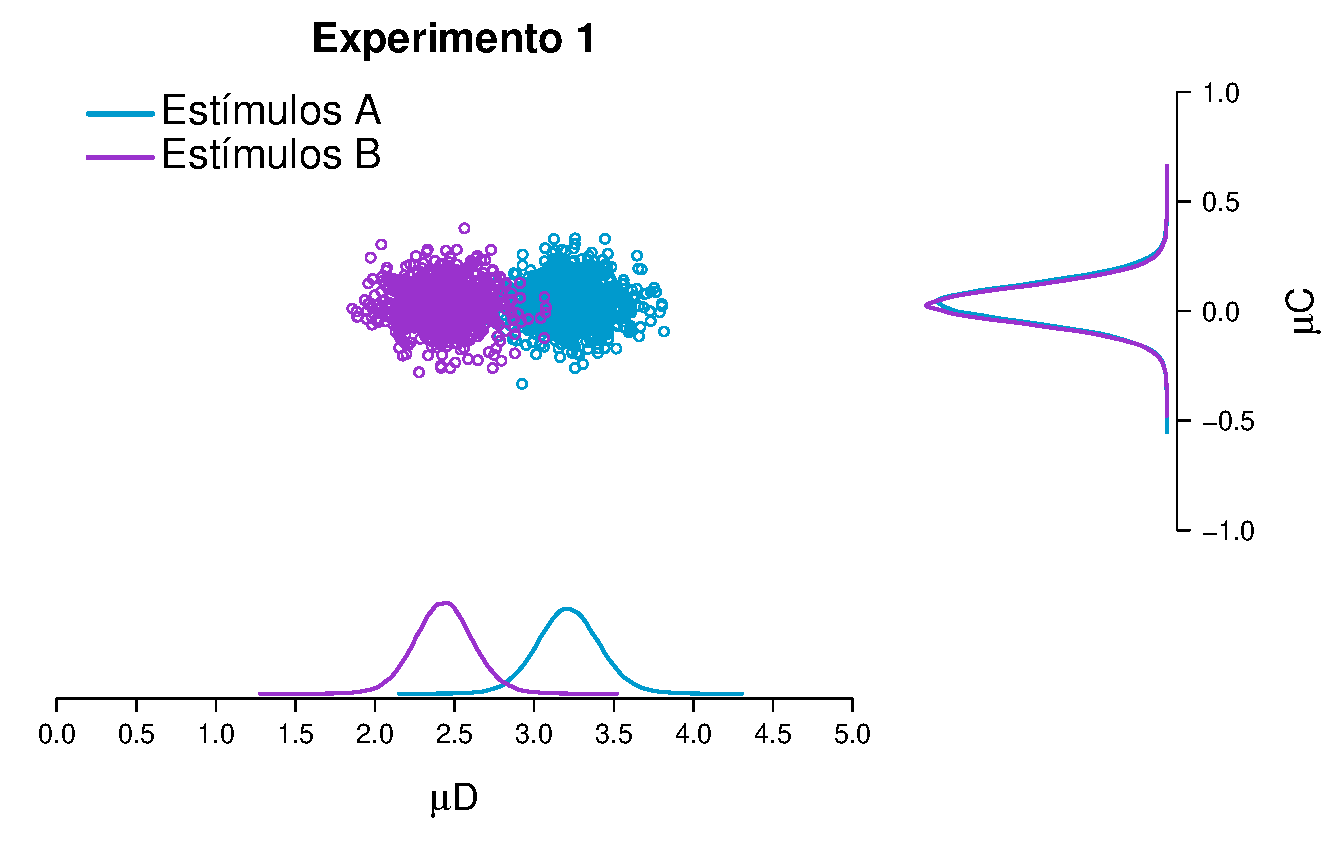
\includegraphics[width=0.7\textwidth]{Figures/MDelta_Joint_E1}\\
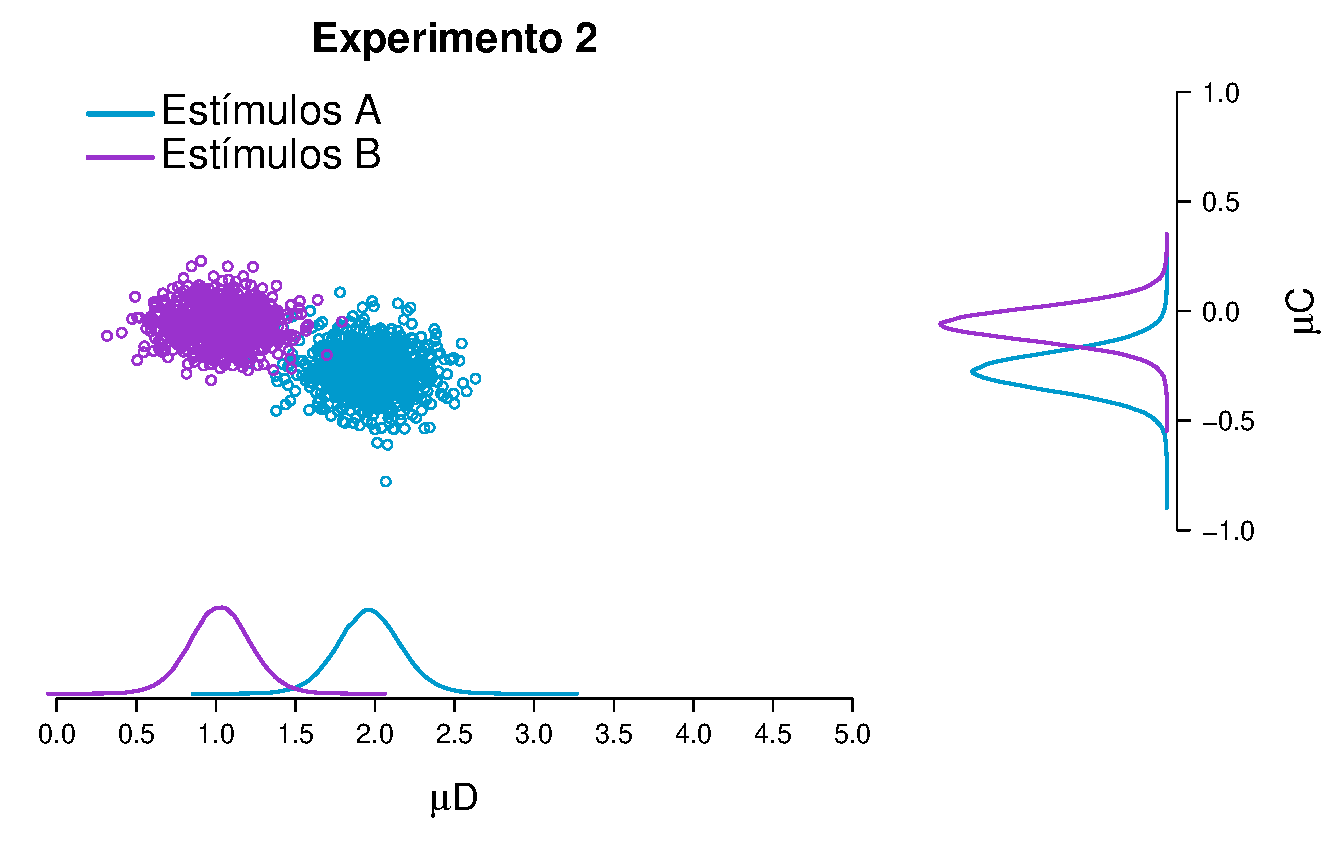
\includegraphics[width=0.7\textwidth]{Figures/MDelta_Joint_E2}\\
%\decoRule
\caption[Modelo Delta: Distribuciones posteriores marginales y conjuntas para las medias de $d'$ y $c$ en cada clase de estímulo]{}
\label{fig:Delta_Joints}
\end{figure}

De acuerdo con la Figura~\ref{fig:Delta_Joints} parece ser que, en general, los valores estimados por el modelo para las medias de $d'$ en cada clase de estímulo son de hecho diferentes. Esto se puede observar tanto en las distribuciones de densidad marginal trazadas por cada clase de estímulo, que se sobrelapan sobre un rango pequeño de valores y con baja probabilidad, como en la distribución de los puntos trazados por cada pareja de valores inferidos de $d'$ y $c$ por cada clase de estímulo, donde se puede distinguir con facilidad dos aglomeraciones de puntos estimados: las inferencias realizadas para la clase A, que tiende a tener valores más bajos de $\mu d'$ y las inferencias sobre la clase B, con valores $\mu d'$ más altos. La distancia entre los valores de $\mu d'(A)$ y $\mu d'(B)$ estimados es mayor en el Experimento 1, donde sólo se presentó una ilusión de Ebbinghaus por ensayo.\\

También es interesante señalar que de acuerdo con las inferencias presentaas en la Figura~\ref{fig:Delta_Joints}, no parece haber diferencias entre los promedios del sesgo $c$ con que los participantes responden a cada clase de estímulos. En particular, en el Experimento 1 se puede observar que los valores estimados para $\mu c$ por cada clase de estímulo se despliegan en un mismo rango de valores, siendo que las distribuciones marginales de densidad posterior se presentan completamente sobrelapadas. Por otro lado, aunque en el Experimento 2 las distribuciones marginales de densidad postrior para $\mu c$ por cada clase de estímulo no se presentan tan iguales como en el Experimento 1, los valores estimados para los estímulos A o B siguen compartiendo un rango de valores relativamente amplio, tomando en cuenta la estrechez de dichas distribuciones.\\

Para evaluar la variabilidad de los valores de $d'$ y $c$ computados por cada participante para cada clase de estímulo, las Figuras~\ref{fig:Delta_Dprima} y \ref{fig:Delta_Cbias} presentan las densidades de probabilidad posterior computadas por cada par de Hits y Falsas Alarmas registrado en cada una de las clases de estímulos. En estas Figuras se presenta además, con una línea más gruesa, la densidad de probabilidad de los valores estimados para las medias de cada parámetro para las clases A y B.\\

\begin{figure}[th]
\centering
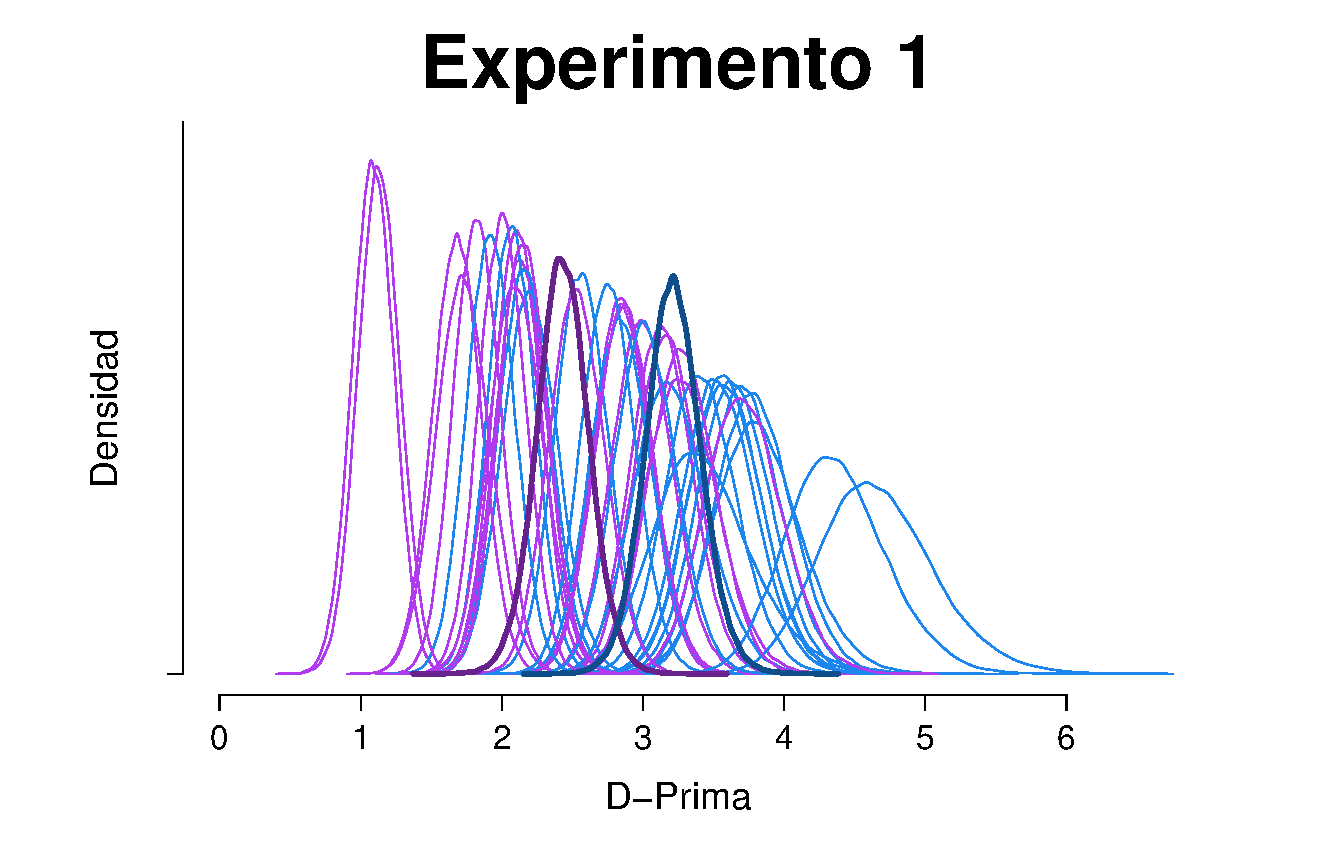
\includegraphics[width=0.6\textwidth]{Figures/MDelta_Dprima_E1}\\
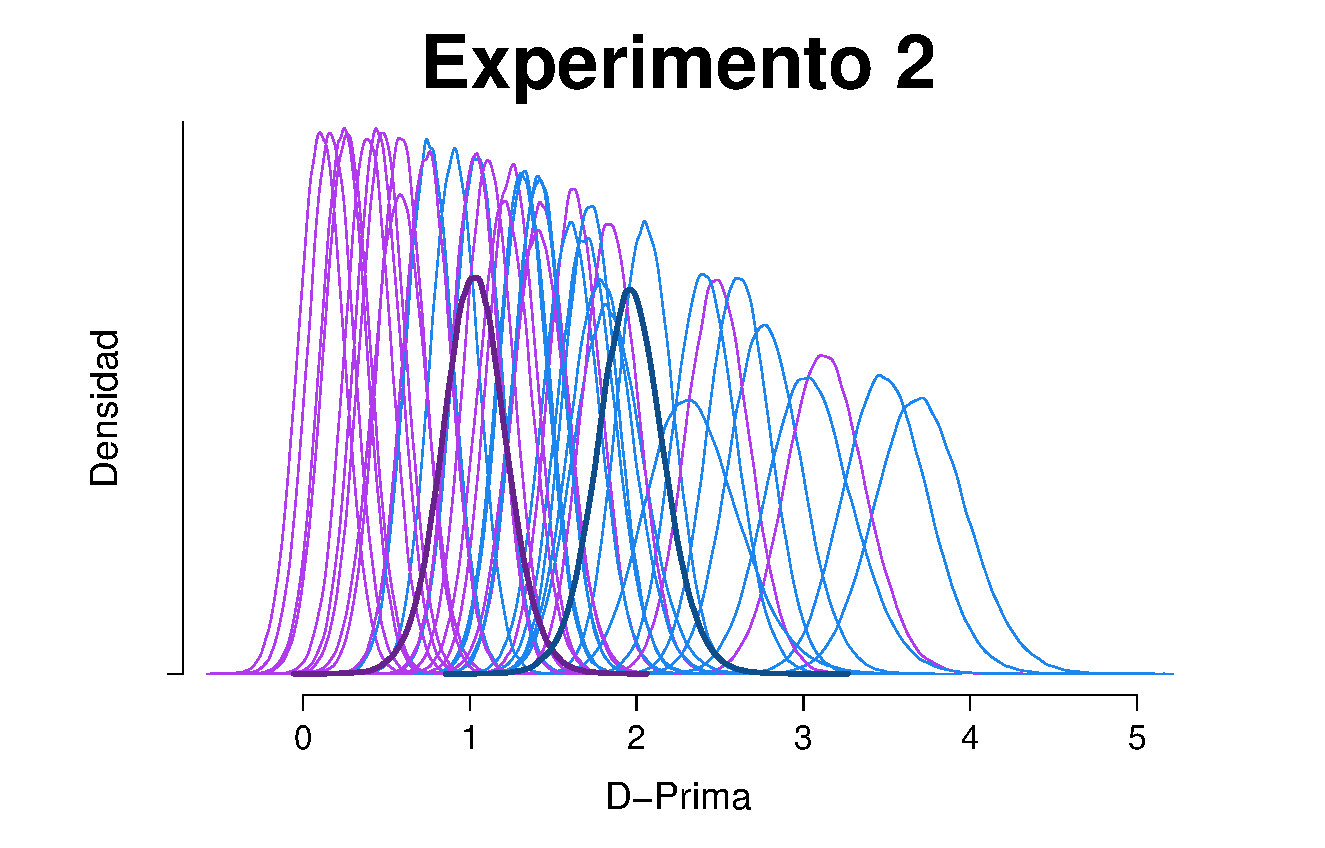
\includegraphics[width=0.6\textwidth]{Figures/MDelta_Dprima_E2}\\
%\decoRule
\caption[Modelo Delta: Distribuciones posteriores conjuntas para las medias de $d'$ y $c$ en cada clase de estímulo]{}
\label{fig:Delta_Dprima}
\end{figure}

En la Figura~\ref{fig:Delta_Dprima} se presentan las estimaciones realizadas por cada participante acerca del valor de $d'$ que mejor describe su desempeño ante cada clase de estímulo, distinguiendo en paneles distintos los valores estimados en el Experimento 1 (panel superior) y 2 (panel inferior). De acuerdo con las densidades de probabilidad posterior estimadas por cada par de Hits y Falsas Alarmas registrado, puede observarse que en el extremo derecho -que corresponde con valores de $d'$ altos que indican una alta discriminabilidad- se encuentran una mayor cantidad de inferencias realizadas para la clase fácil A, en tanto que en el extremo izquirdo -valores bajos de $d'$ que sugieren una baja discriminabilidad- se concentra una mayor cantidad de distribuciones de densidad correspondientes al cómputo realizado apra la clase difícil B. De manera adicional, la figura presenta con líneas más gruesas los valores estimados para las medias de $d'$ en cada condición, permitiendo que su exploración sea realizada a la luz de la variabilidad capturada por las estimaciones individuales.\\

\begin{figure}[th]
\centering
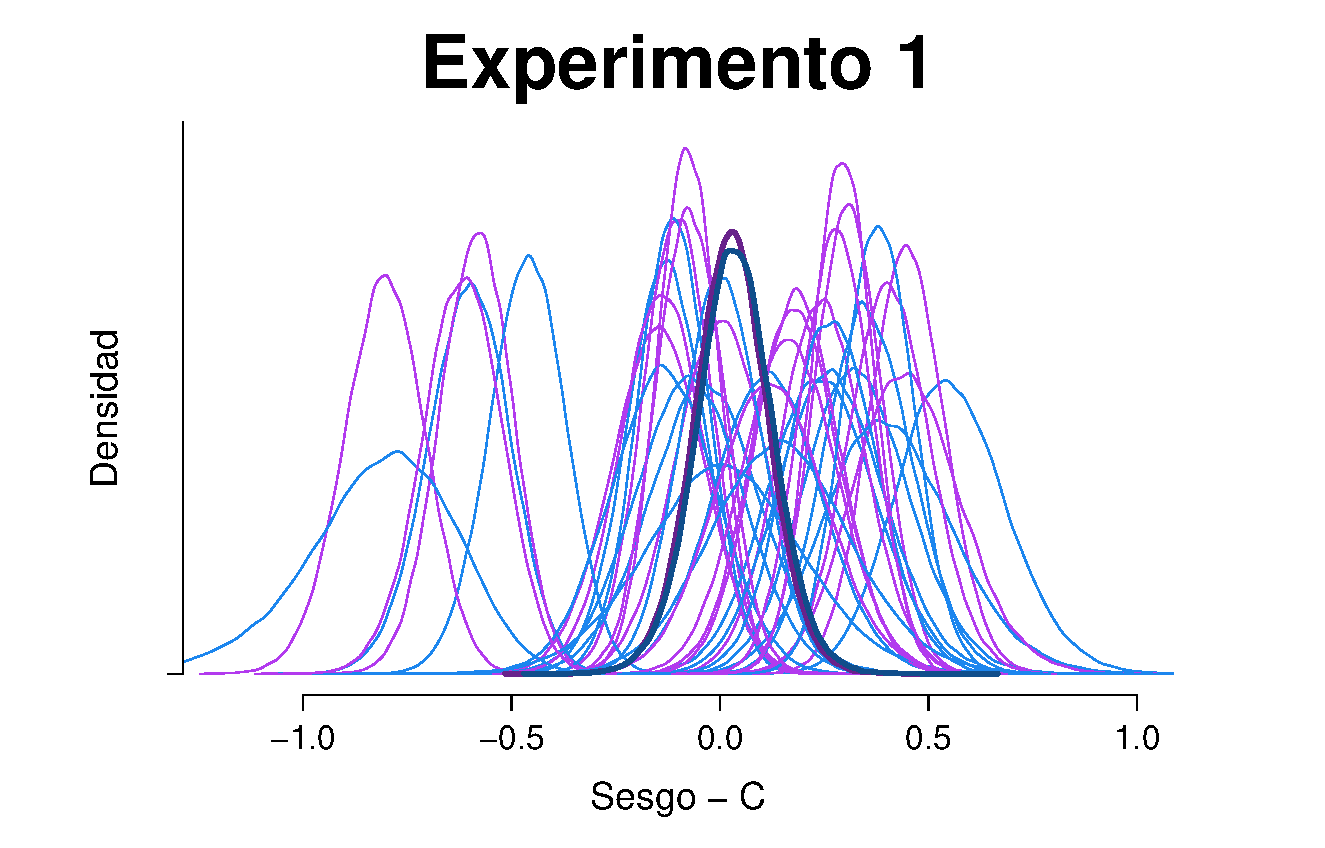
\includegraphics[width=0.6\textwidth]{Figures/MDelta_Cbias_E1}\\
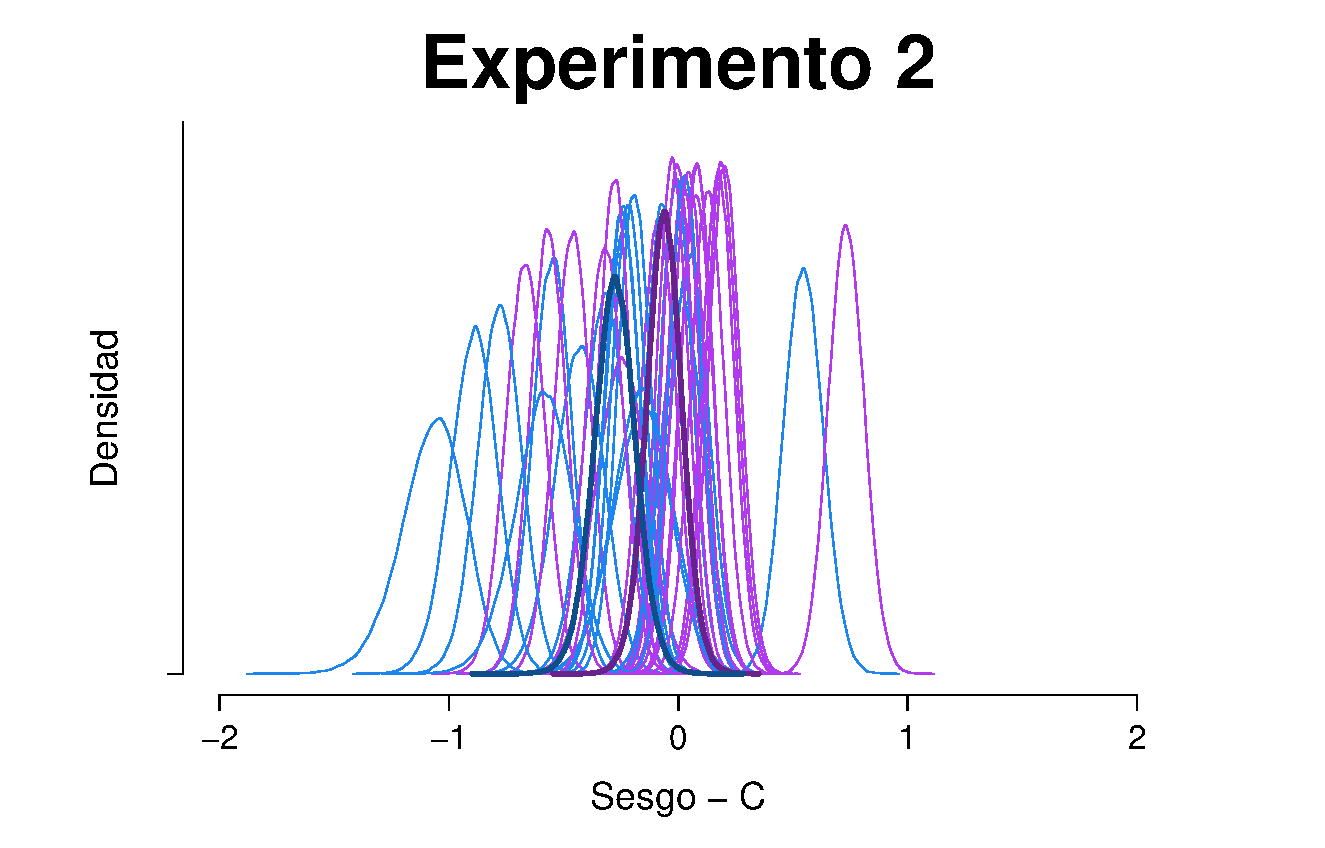
\includegraphics[width=0.6\textwidth]{Figures/MDelta_Cbias_E2}\\
%\decoRule
\caption[Modelo Delta: Distribuciones posteriores conjuntas para las medias de $d'$ y $c$ en cada clase de estímulo]{}
\label{fig:Delta_Cbias}
\end{figure}

Por su parte, en cuanto a los valores del parámetro $c$ estimados por cada participante, en la Figura~\ref{fig:Delta_Cbias} se pueden apreciar diferencias en términos de las inferencias realizadas a partir de los datos recopilados en cada experimento. En el Experimento 1, pese a la variabilidad en las estimaciones realizadas, no parece haber ninguna relación entre el tipo de estímulo y los valores de $c$ estimados, tal y como se ilustra con el sobrelape total en que se presentan las densidades de probabilidad posterior estimadas para las medias de ambos grupos. Por otro lado, en el caso del Experimento 2 sí parece haber una ligera diferencia en términos del sesgo con que los participantes responden a cada clase de estímulos, siendo que en general se observan valores de $c$ por debajo de 0 (sesgo liberal) en los estímulos de la clase A, mientras que en la clase B se observa la misma ausencia de sesgo ($c$ cercano a $0$) que en los estímulos presentados en el Experimento 1.\\

Finalmente, la Figura~\ref{fig:Delta} presenta la densidad de probabilidad posterior computada para las diferencias entre las medias de $d'$ computadas por cada condición, que se traducen en distintos valores del parámetro $\delta$. Tal como se puede apreciar en la figura, parece ser que a la luz de los datos registrados en los dos experimentos realizados, es muy poco probable que la diferencia entre las $d'$ asociadas a cada clase de estímulo sea 0. De acurdo con las gráficas presentadas, los picos más altos de densidad de probabilidad aparecen cerca de 1, lo que sugeriría que la media de las $d'$ asociadas a cada clase de estíimulos difieren al rededor de una unidad de desviación estándar.\\

\begin{figure}[th]
\centering
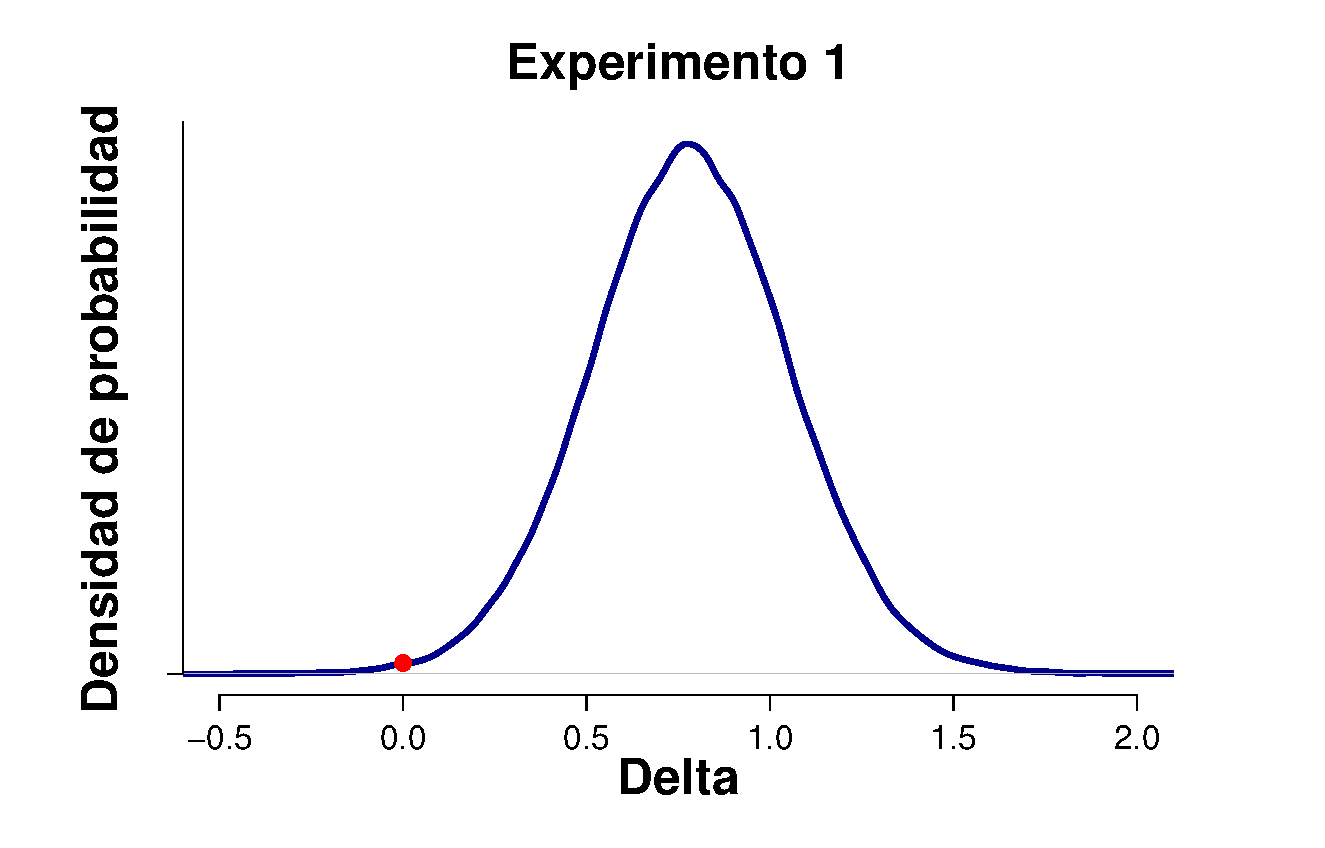
\includegraphics[width=0.6\textwidth]{Figures/MDelta_DensidadDelta_E1}\\
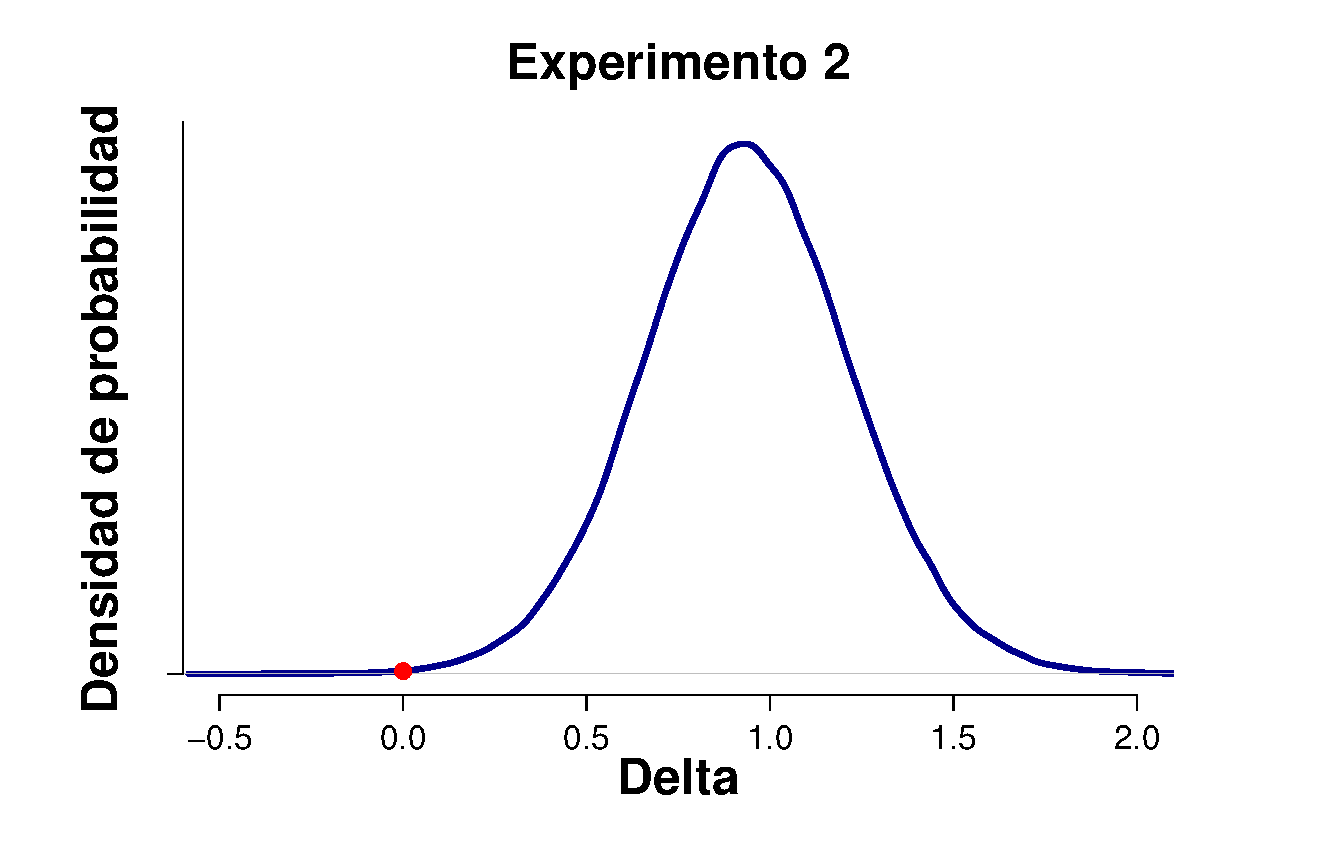
\includegraphics[width=0.6\textwidth]{Figures/MDelta_DensidadDelta_E2}\\
%\decoRule
\caption[Modelo Delta: Densidad de probabilidad posterior para el valor del parámetro Delta]{Modelo jerárquico bayesiano desarrollado a partir del supuesto de que los valores de $d'$ y sesgo $c$ computados por cada participante en cada clase provienen de su propia distribución normal. El modelo incorpora un parámetro ($\delta$) que estima la diferencia entre las medias de $d'$ estimadas por cada condición. El modelo tiene priors no informativas.}
\label{fig:Delta}
\end{figure}

En conjunto, los análisis de datos realizados arrojaron evidencia a favor de la manipulación experimental implementada en el diseño de los estímulos diseñados para formar los dos niveles de dificultad a comparar. Se confirmó la existencia de una diferencia significativa en la discriminabilidad ($d'$) asociada a cada clase de estímulos, que además se reportó de acuerdo a lo esperado con base en la literatura revisada para el diseño de los estímulos: las figuras de Ebbinghaus compuestas por un número menor de círculos externos (clase A), tuvieron valores de $d'$ más grandes que las figuras de la clase B, formados por un número mayor de círculos externos.\\

Una vez comprobada la relación $d'(A) > d'(B)$, se prosiguió a evaluar la presentación de los patrones de respuesta identificados como Efecto Espejo en Memoria de Reconocimiento, en los datos obtenidos en el presente trabajo.\\












\subsection{Diferencias en las Tasas de Hits y Falsas Alarmas}

Como se recordará de la revisión presentada en el Capítulo 1 acerca del fenómeno identificado como Efecto Espejo en Memoria de Reconocimiento, la evidencia en favor del mismo se presenta en Tareas de respuesta binaria "Sí/No" a partir de la siguiente relación:\\
 
\begin{center}
$FA(A) < FA(B) < H(B) < H(A)$\\
\end{center}
\begin{center}
donde $FA$ y $H$ señalan las tasas de Hits y Falsas Alarmas observadas durante la tarea en cada clase, \parencite{Glanzer1993}.\\
\end{center}

Para comprobar que esta misma relación se presentara en los datos obtenidos en el presente estudio, se comparó el número de Hits y Falsas Alarmas cometidos en cada una de las clases de estímulos construidas por cada participante.\\

Una forma sencilla de explorar dicha relación fue mediante la realización de gráficas de barras que presentaran las diferencias en los resultados obtenidos por los participantes para los distintos tipos de estímulos presentados. Como un caso ejemplar, en la Figura~\ref{fig:MirrorRate_E2_P4} se muestra la frecuencia absoluta de Hits y Falsas Alarmas obtenidas por el Participante 4 en el Experimento 2, por cada clase de estímulos construido, distinguiendo la clase fácil A en color azul y la clase difícil B, en púrpura. Como se puede apreciar, dicho participante presentó el patrón de respuestas identificado como Efecto Espejo.\\

\begin{figure}[th]
\centering
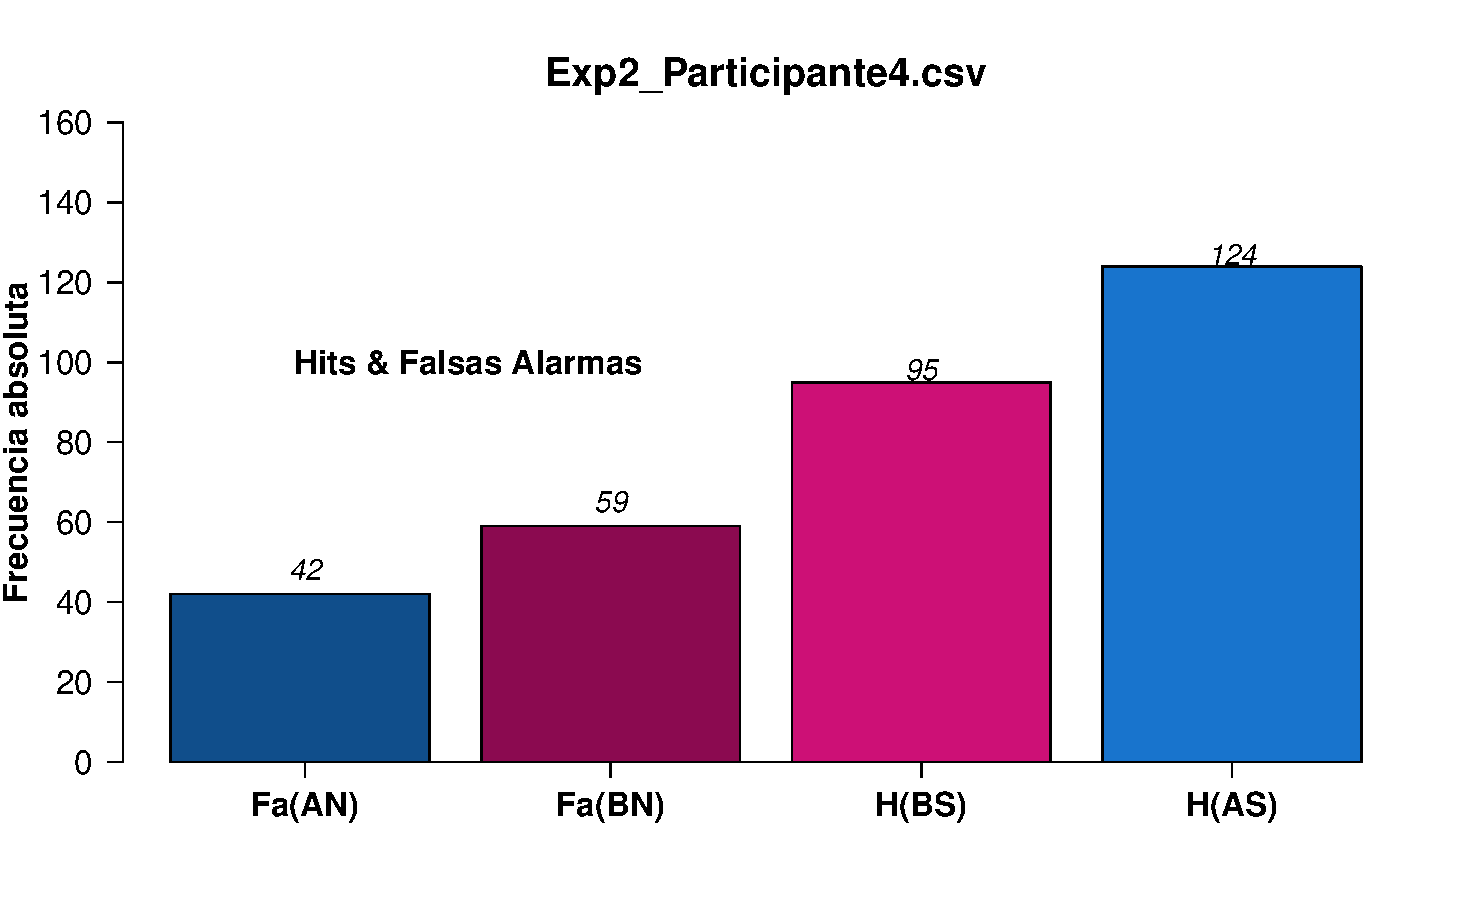
\includegraphics[width=0.60\textwidth]{Figures/MirrorRate_Exp2_P4}
%\decoRule
\caption[Diferencias entre Hits y Falsas Alarmas por Condición; Participante ejemplar]{Se muestra el desempeño del Participante 14 del Experimento 2 en relación al color de los estímulos. En el panel izquierdo se muestra la relación entre el número de Hits obtenidos y el color de los estímulos, mientras que en el panel derecho se muestra la misma relación para las Falsas alarmas.}
\label{fig:MirrorRate_E2_P4}
\end{figure}

Las gráficas correspondientes al desempeño del resto de los participantes en los Experimentos 1 y 2, pueden consultarse en los Apéndices.\\

La comparación global entre las tasas de Hits y Falsas Alarmas registradas por cada participante de los Experimentos 1 y 2 en cada tipo de estímulo se presenta en la Figura~\ref{fig:Diff_Rate}. De acuerdo con el patrón de respuestas reportado como parte del Efecto Espejo, se espera observar una pendiente descendente para la comparación de las tasas de Hits registradas por cada condición (paneles izquierdos) y una pendiente ascendente en el registro de tasas de Falsas Alarmas (paneles derechos). Como se puede observar, parece ser que dichas tendencias se aparecen en la mayoría de los participantes, presentándose de manera más evidente en los datos registrados en el Experimento 1. Sin embargo, resulta poco claro si las diferencias entre las tasas registradas en una y otra clase de estímulos son lo suficientemente grandes como para considerarse estadísticamente significativas.\\

\begin{figure}[th]
\centering
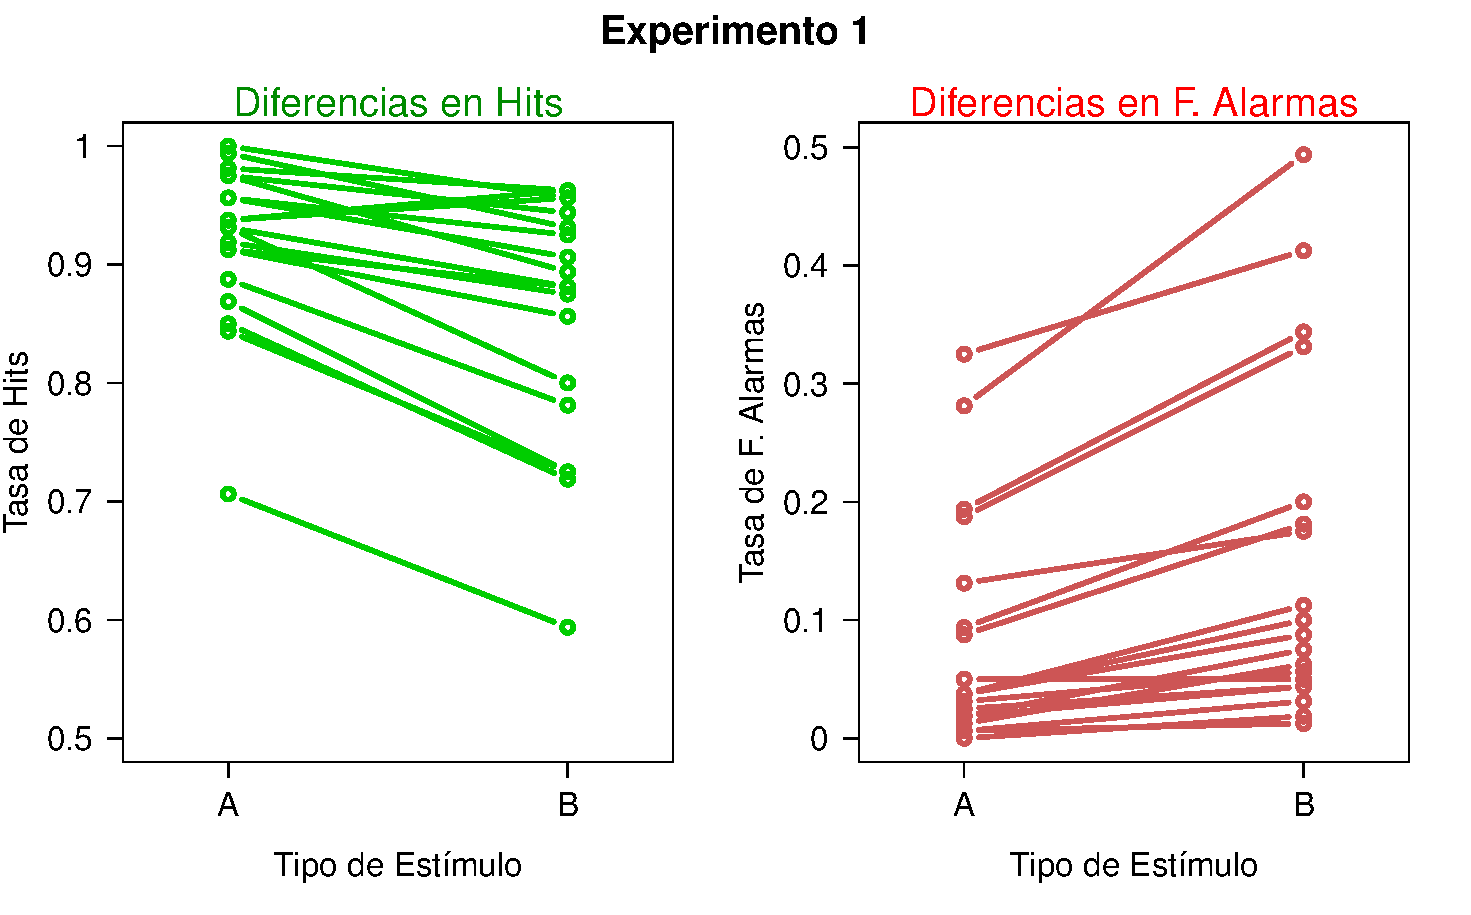
\includegraphics[width=0.80\textwidth]{Figures/Diff_Rate_E1}\\ 
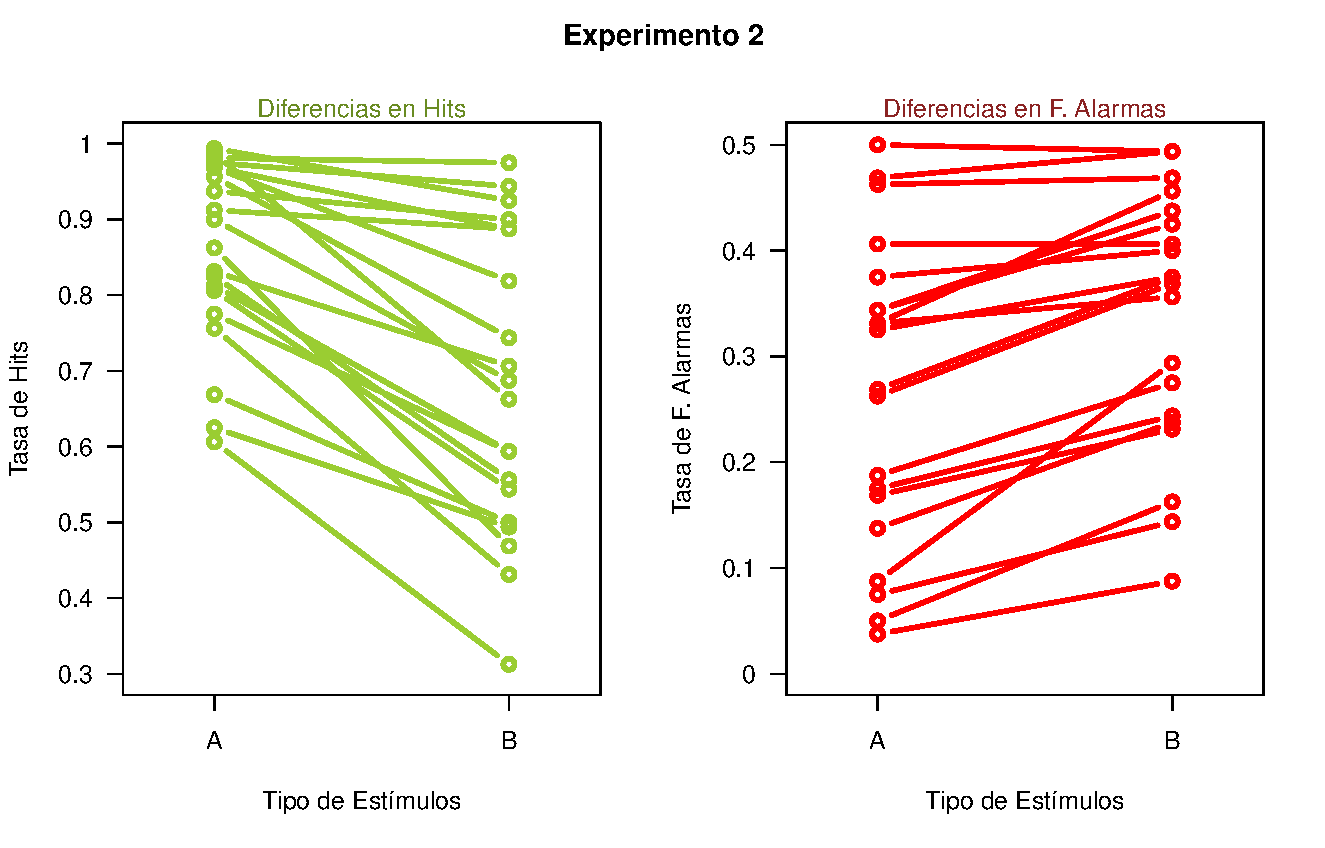
\includegraphics[width=0.80\textwidth]{Figures/Diff_Rate_E2}
%\decoRule
\caption[Diferencias entre las Tasas de Hits y Falsas Alarmas registradas en cada clase de estímulos]{Se presenta la comparación, participante a participante, entre las tasas de Hits y Falsas Alarmas registradas para cada clase de estímulo, (paneles izquierdos y derechos, respectivamente). El panel superior muestra las comparaciones correspondientes al Experimento 1 y el panel inferior, al Experimento 2.}
\label{fig:Diff_Rate}
\end{figure}

A continuación se presentan los análisis realizados para determinar si los Hits y las Falsas Alarmas registrados por cada clase de estímulos son estadísticamente diferentes.\\

\textbf{Análisis 1: Pruebas T para comparar las tasas de Hits y Falsas Alarmas registradas por cada clase de estímulos}\\

De acuerdo con la literatura, la manera más apropiada de evaluar la significancia estadística del patrón de respuestas reportado como Efecto Espejo en Tareas de respuesta binaria "Sí/No", es mediante la realización de dos pruebas-T que evalúen de manera independiente las diferencias entre las medias de las tasas de Hits reportadas por cada clase de estímulo y entre las tasas de Falsas Alarmas, \parencite{Glanzer1990}.\\

Sin embargo, debido que los datos a comparar entre las clases de estímulos presentados son tasas, sólo pueden adoptar valores entre $0$ y $1$ 

a Tabla~\ref{Tabla_t-HitsyFA}\\


\begin{table}
\caption[Prueba T para evaluar diferencias en las medias de las tasas de ejecución (Hits y F. Alarmas) entre condiciones]{Diferencias en Hits y Falsas Alarmas entre los tipos de estímulos (Experimento 1 y 2)}
\label{Tabla_t-HitsyFA}
\centering
\begin{tabular}{l l | c c c c c c}
\toprule
%\tabhead{Groups} & \tabhead{Treatment X} & \tabhead{Treatment Y} \\
\textbf{Experimento} & \textbf{Tasa} & \textbf{$\mu(A)$} & \textbf{$arcsin(\mu(B))$} & \textbf{$\mu(A)$} & \textbf{$arcsin(\mu(B))$} &\textbf{T} & \textbf{P value}\\
\midrule
Exp 1 & Hits & 0.922 & 1.314 & 0.860 & 1.209 & -2.4348 & 0.0098 \\
Exp 1 & FA & 0.08 & 0.247 & 0.143 & 0.353 & 1.872 & 0.0345 \\
Exp 2 & Hits & 0.857 & 1.219 & 0.681 & 0.994 & -3.3595, & 0.0009 \\
Exp 2 & FA & 0.266 & 0.524 & 0.336 & 0.611 & 1.7223 & 0.0468 \\
\bottomrule
\end{tabular}
\end{table}

\textbf{Modelo bayesiano}


\begin{figure}[th]
\centering
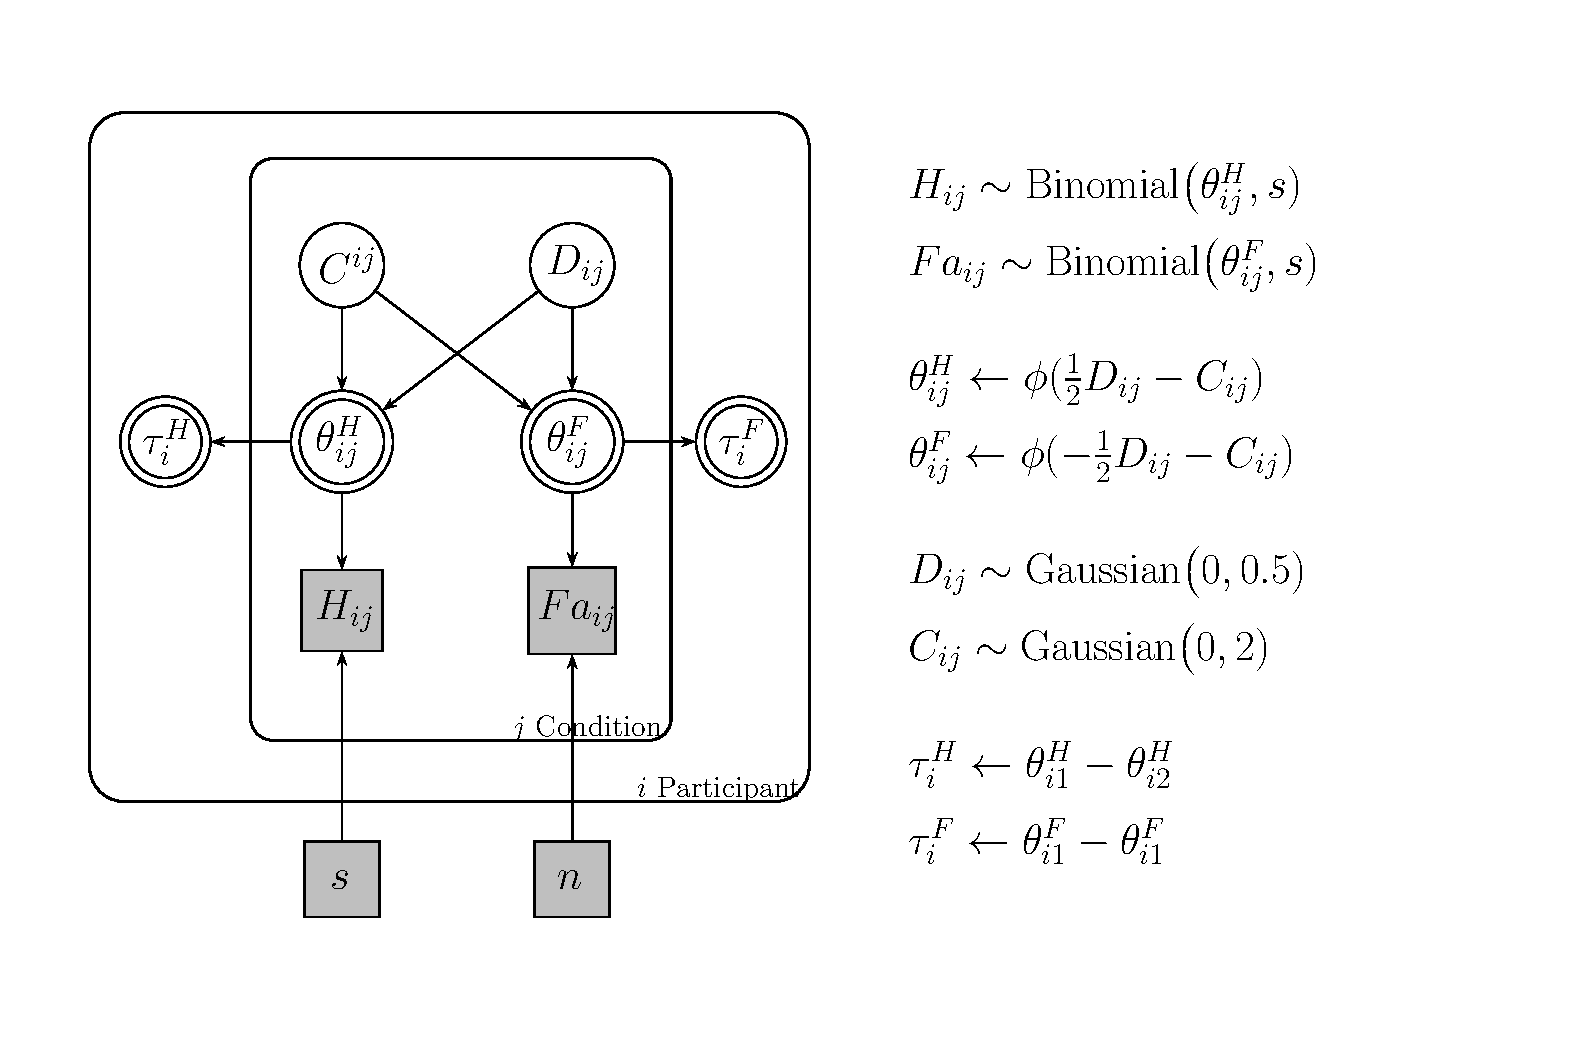
\includegraphics[width=1.1\textwidth]{Figures/Model_Tau_Diff_Tetas}
%\decoRule
\caption[Modelo Tau: Modelo Bayesiano para evaluar las diferencias entre las tasas de hits y falsas alarmas]{Comparación intrasujeto de}
\label{fig:Mod_Tau}
\end{figure}














\subsection{Diferencias en la asignación de Puntajes de Confianza}


La Figura~\ref{fig:MirrorRating_E1_P10} muestra el promedio de los puntajes de confianza asignados por el Participante 10 del Experimento 1 a los estímulos pertenecientes a cada una de las condiciones de dificultad construidas, separando para cada caso los ensayos con ruido y señal. En la figura puede apreciarse con claridad una tendencia ascendente que coincide con el patrón reportado en estudios de Memoria de Reconocimiento.\\

\begin{figure}[th]
\centering
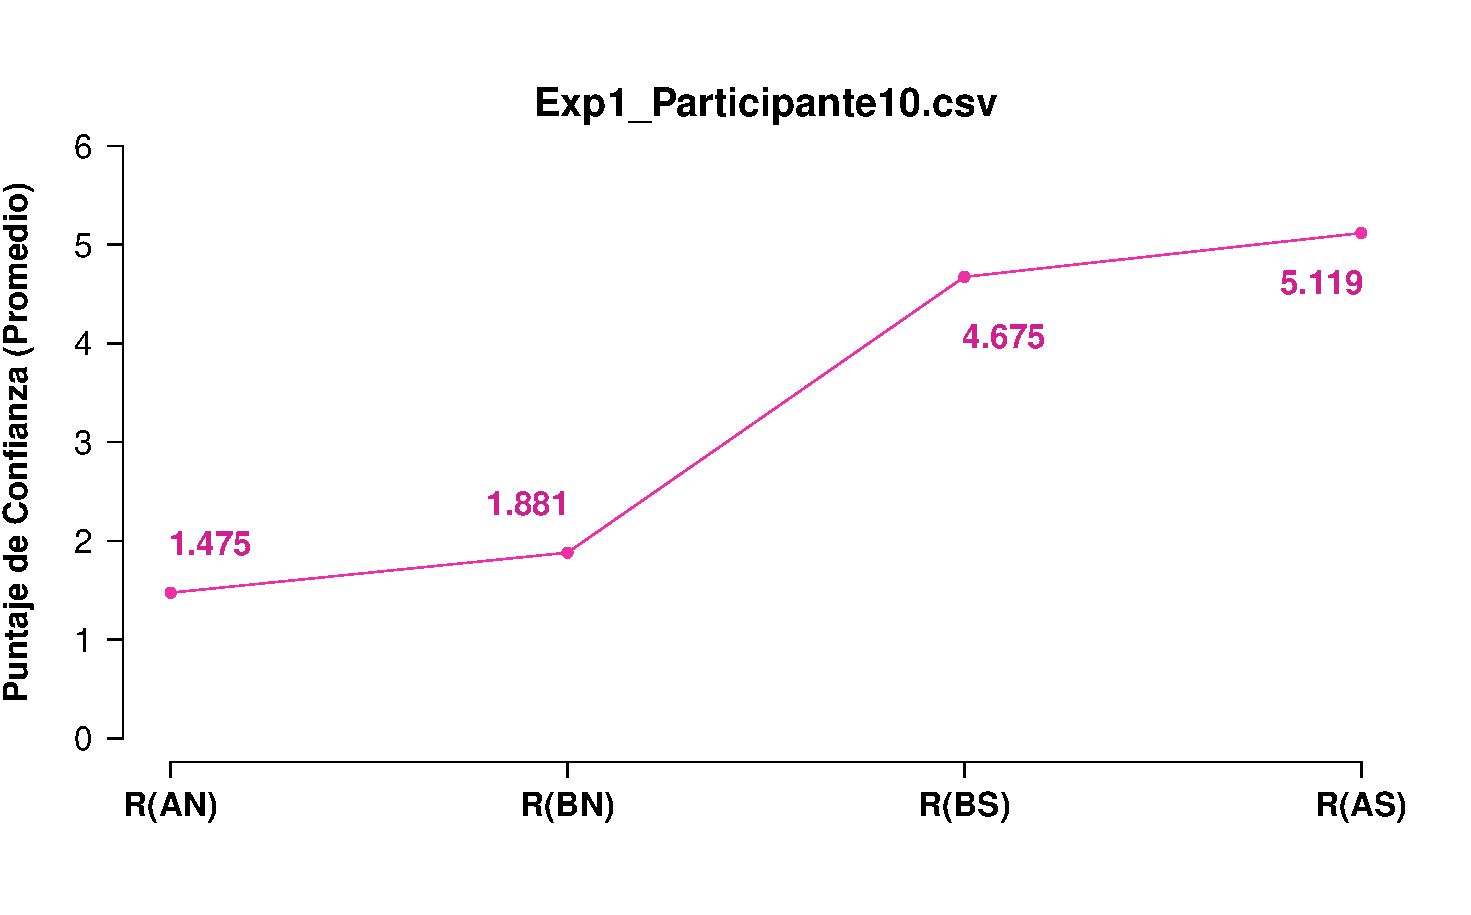
\includegraphics[width=0.60\textwidth]{Figures/MirrorRating_Exp1_P10}
%\decoRule
\caption[Comparación entre Puntajes de Confianza asignados por Condición; Ejemplo]{Se muestra el desempeño del Participante 14 del Experimento 1 en relación al color de los estímulos. En el panel izquierdo se muestra la relación entre el número de Hits obtenidos y el color de los estímulos, mientras que en el panel derecho se muestra la misma relación para las Falsas alarmas.}
\label{fig:MirrorRating_E1_P10}
\end{figure}

%La comparación entre los puntajes de confianza asignados a cada grupo de estímulos por el resto de los participantes en los Experimentos 1 y 2, se presentan en las Figuras~\ref{fig:MERating_E1} y ~\ref{fig:MERating_E2}.\\





\textbf{Análisis 1: }

\begin{table}
\caption[Prueba T para evaluar diferencias en las medias de los puntajes de confianza asigandos entre condiciones]{}
\label{Tabla_t-HitsyFA}
\centering
\begin{tabular}{l l |  c c c c}
\toprule
%\tabhead{Groups} & \tabhead{Treatment X} & \tabhead{Treatment Y} \\
\textbf{Experimento} & \textbf{Ensayo} & \textbf{$\mu$ A} & \textbf{$\mu$ B} & \textbf{T} & \textbf{P value}\\
\midrule
Exp 1 & Signal & 5.445 & 5.212 & -1.7778, & 0.0418 \\
Exp 1 & Noise & 1.542 & 1.883 & -1.7208 & 0.0472 \\
Exp 2 & Signal & 5.183 & 4.342  & -3.6752, & 0.0004 \\
Exp 2 & Noise & 2.386 & 2.752 & -1.809 & 0.0391 \\
\bottomrule
\end{tabular}
\end{table}


\textbf{Análisis Bayesiano: Prueba T bayesiana }











\subsection{Réplica de controles reportados en la literatura}



